% ===========================================================
% บทที่ 2: เอกสารและงานวิจัยที่เกี่ยวข้อง
% ===========================================================

% -----------------------------------------------------------
\section{งานวิจัยด้านการถ่ายโอนทรงผมด้วยเทคนิคปัญญาประดิษฐ์}
% -----------------------------------------------------------

ก่อนเลือกโมเดลมาใช้ ผู้วิจัยได้ทบทวนงานด้านการถ่ายโอนทรงผมและสีผม
(Hair Transfer)~\cite{Zhu_2021,nikolaev2024hairfastganrealisticrobusthair} ที่ผ่านมา
เพื่อดูว่าแต่ละแนวทางแก้ปัญหาใดได้แล้ว และยังมีข้อจำกัดอะไร
งานเหล่านี้แบ่งได้เป็น 3 กลุ่ม กลุ่มแรกคือโมเดลโครงข่ายปรปักษ์เชิงกำเนิด
(Generative Adversarial Network: GAN)~\cite{goodfellow2014generativeadversarialnetworks}
ที่หารหัสของภาพด้วยการปรับค่าซ้ำหลายรอบ (Optimization-based) ซึ่งได้ภาพดีแต่ช้า
กลุ่มที่สองคือโมเดล GAN ที่ใช้ตัวเข้ารหัส (Encoder-based) คำนวณรหัสออกมาในครั้งเดียว ซึ่งเร็วแต่มักเสียรายละเอียด
และกลุ่มที่สามคือแบบจำลองดิฟฟิวชัน (Diffusion-based) ที่วาดรายละเอียดได้ดี แต่ควบคุมผลได้ยากและใช้เวลามากกว่า
หัวข้อนี้เล่าถึงงานแต่ละชิ้นตามลำดับที่แนวคิดพัฒนาต่อกันมา

งานแรกที่ควรรู้จักคือ StyleGAN2 (Style-based Generative Adversarial Network รุ่นที่ 2)
ของ Karras และคณะ~\cite{karras2020analyzingimprovingimagequality} เพราะทั้ง Barbershop และ HairFastGAN ใช้ StyleGAN2 เป็นตัววาดภาพ
StyleGAN2 เป็นโมเดลที่รับตัวเลขชุดหนึ่ง (เรียกว่ารหัส $w$) แล้ววาดออกมาเป็นภาพใบหน้าคน
โดยเริ่มวาดจากภาพขนาดเล็ก $4 \times 4$ พิกเซล แล้วขยายขึ้นทีละขั้นจนได้ภาพขนาด $1024 \times 1024$ พิกเซล
รหัสที่ต่างกันจะได้ใบหน้าที่ต่างกัน StyleGAN2 พัฒนาต่อจาก StyleGAN รุ่นแรก~\cite{karras2019stylebasedgeneratorarchitecturegenerative}
ซึ่งมักมีจุดเพี้ยนในภาพ จนได้ภาพที่สมจริงมาก
โดยมีค่า Fréchet Inception Distance (FID) เท่ากับ 2.84 บนชุดภาพใบหน้า Flickr-Faces-HQ (FFHQ)
ค่า FID วัดว่าภาพที่สร้างขึ้นมีลักษณะโดยรวมใกล้กับภาพจริงเพียงใด ยิ่งต่ำยิ่งดี
ข้อจำกัดของ StyleGAN2 คือ ถ้าต้องการแก้ไขภาพถ่ายจริงของคนคนหนึ่ง ต้องหาให้ได้ก่อนว่าภาพนั้นตรงกับรหัสใด
ขั้นตอนนี้เรียกว่าการแปลงภาพกลับเป็นรหัสแฝง (GAN Inversion)

Barbershop ของ Zhu และคณะ~\cite{Zhu_2021} เป็นงานเปลี่ยนทรงผมที่ถูกอ้างถึงมาก
แนวคิดหลักคือแยกรหัสของภาพออกเป็น 2 ส่วน ส่วนแรก $F$ (Structure Tensor) เก็บข้อมูลว่าสิ่งใดอยู่ตรงไหนในภาพ เช่น ผมอยู่บริเวณใด
ส่วนที่สอง $S$ (Appearance Code) เก็บข้อมูลว่าแต่ละส่วนมีลักษณะอย่างไร เช่น ผมสีอะไร
ทั้งสองส่วนรวมกันเรียกว่าพื้นที่แฝง $FS$ (FS Latent Space)
เมื่อแยกได้แบบนี้ จึงนำ ``ตำแหน่งของผม'' จากภาพหนึ่ง และ ``สีผม'' จากอีกภาพหนึ่งมาประกอบกันได้
โดยใบหน้ายังเป็นของคนเดิม
ขั้นตอนโดยสรุปคือ แบ่งส่วนภาพด้วยหน้ากาก (Segmentation Mask)
ซึ่งเป็นภาพที่ระบุว่าพิกเซลใดเป็นผม ใบหน้า หรือพื้นหลัง แล้วแปลงทุกภาพเป็นรหัส $FS$
ปรับรหัสให้ผมอยู่ตามหน้ากากเป้าหมาย แล้วให้ StyleGAN2 วาดภาพใหม่
ผลที่ได้คือภาพที่สมจริงมาก ในการทดสอบกับผู้ใช้ ผู้ใช้เลือกภาพของ Barbershop มากกว่าภาพของวิธีเดิมประมาณร้อยละ 95--96
แต่เพราะต้องค้นหารหัสซ้ำหลายร้อยรอบกับทุกภาพ จึงใช้เวลาประมาณ 3.5--10.8 นาทีต่อภาพ
ซึ่งนานเกินไปสำหรับการใช้งานที่ผู้ใช้ต้องรอผล

Style Your Hair ของ Kim และคณะ~\cite{kim2022stylehairlatentoptimization} แก้ปัญหาของ Barbershop
ในกรณีที่คนในภาพใบหน้ากับคนในภาพทรงผมหันหน้าไปคนละทาง (ท่าทางหรือ Pose ต่างกัน) ซึ่ง Barbershop มักวางผมผิดตำแหน่ง
โดยเพิ่มค่าสูญเสีย (Loss) ซึ่งเป็นตัวเลขที่บอกว่าผลลัพธ์ยังห่างจากสิ่งที่ต้องการเพียงใด อีก 2 ตัว
ได้แก่ ค่าสูญเสียที่ช่วยจัดท่าทางจากจุดสำคัญบนใบหน้าแบบสามมิติ (Pose Align Loss)
และค่าสูญเสียที่รักษาลวดลายของผมเฉพาะจุด (Local-Style-Matching Loss)
วิธีนี้ได้ค่า FID 17.06 ซึ่งดีกว่า Barbershop (18.07) แต่ยังเป็นการค้นหาแบบปรับค่าซ้ำ จึงยังช้า ประมาณ 3--4 นาทีต่อภาพ

HairCLIP ของ Wei และคณะ~\cite{wei2022hairclipdesignhairtext} ให้ผู้ใช้สั่งเปลี่ยนผมได้ด้วยข้อความ
เช่น พิมพ์ว่า ``ผมหยิกสีบลอนด์'' หรือจะใช้ภาพอ้างอิงก็ได้
งานนี้อาศัย CLIP (Contrastive Language-Image Pre-training)~\cite{radford2021learningtransferablevisualmodels}
ซึ่งเป็นโมเดลที่เข้าใจทั้งภาพและข้อความในพื้นที่เดียวกัน แล้วใช้เครือข่ายขนาดเล็ก (Mapper)
ปรับรหัส $W^{+}$ ของ StyleGAN (รหัสแฝงแบบหนึ่ง ซึ่งอธิบายในหัวข้อที่~\ref{sec:stylegan2}) ตามคำสั่ง
จุดเด่นคือเร็วมาก ใช้เวลา 0.10--0.36 วินาทีต่อภาพ
และภาพผลลัพธ์ยังคล้ายภาพเดิม (ดัชนีความคล้ายเชิงโครงสร้าง หรือ Structural Similarity Index Measure: SSIM ประมาณ 0.92)
แต่รายละเอียดของเส้นผมมักหายไป
ต่อมามี HairCLIPv2~\cite{wei2023hairclipv2unifyinghairediting} ที่รวมวิธีสั่งงานหลายแบบไว้ในระบบเดียว
ทั้งข้อความ หน้ากาก ภาพร่าง และภาพอ้างอิง โดยใช้การผสมคุณลักษณะจากภาพตัวแทน (Proxy Feature Blending)
ทำให้รักษาพื้นหลังและใบหน้าได้ดีขึ้น (อัตราส่วนสัญญาณสูงสุดต่อสัญญาณรบกวน หรือ Peak Signal-to-Noise Ratio: PSNR ประมาณ 29.5 dB)
แต่ถ้าสั่งด้วยข้อความจะใช้เวลานานขึ้นเป็น 0.5--58.9 วินาที

HairFastGAN ของ Nikolaev และคณะ~\cite{nikolaev2024hairfastganrealisticrobusthair} ตั้งใจแก้ปัญหาความช้าของ Barbershop
แทนที่จะค้นหารหัสซ้ำกับทุกภาพ HairFastGAN ฝึกเครือข่ายตัวเข้ารหัส (Encoder) ไว้ล่วงหน้า ให้คำนวณรหัสออกมาได้ในครั้งเดียว
โดยยังทำงานบนพื้นที่ $FS$ เหมือน Barbershop และเพิ่มตัวหมุนรหัส (Rotate Encoder)
ที่หมุนผมในภาพอ้างอิงให้หันตามใบหน้า กับโมดูลปรับรายละเอียด (Refinement Alignment)
ที่ดึงรายละเอียดของใบหน้าจริงกลับมา ผลคือทำงานเร็วมาก ประมาณ 0.41 วินาทีต่อภาพบนหน่วยประมวลผลกราฟิก
(Graphics Processing Unit: GPU) รุ่น A100 และได้ค่า FID 13.12 ซึ่งดีที่สุดในกลุ่มที่เปรียบเทียบ
แต่ยังทำทรงที่ซับซ้อน เช่น ผมเปียหรือหางม้า ได้ไม่ดี
นอกจากนี้ยังไม่มีงานใดนำ HairFastGAN และ Barbershop มาปรับจูนด้วยข้อมูลและเงื่อนไขเดียวกันเพื่อเปรียบเทียบกันโดยตรง

โมเดลกลุ่ม GAN ข้างต้นมีจุดอ่อนร่วมกัน คือผมที่ได้มักดูนุ่มและเบลอ ไม่เห็นเป็นเส้นชัดเหมือนภาพถ่าย
ผู้วิจัยจึงศึกษาอีกแนวทางหนึ่งคือแบบจำลองดิฟฟิวชัน งานของ Rombach และคณะ~\cite{rombach2022highresolutionimagesynthesislatent}
เสนอแบบจำลองดิฟฟิวชันในพื้นที่แฝง (Latent Diffusion Model: LDM) ซึ่งเป็นพื้นฐานของ Stable Diffusion
แบบจำลองดิฟฟิวชันสร้างภาพโดยเริ่มจากภาพที่มีแต่สัญญาณรบกวน (Noise) แล้วค่อย ๆ ลบสัญญาณรบกวนออกทีละขั้นจนได้ภาพ
ปัญหาของแบบจำลองรุ่นก่อนคือทำงานบนภาพขนาดเต็ม จึงต้องคำนวณมาก
LDM แก้ปัญหานี้โดยบีบภาพให้เล็กลงก่อนด้วยตัวเข้ารหัสอัตโนมัติ (Autoencoder)
แล้วจึงลบสัญญาณรบกวนบนภาพที่บีบแล้ว ด้วยโครงข่ายรูปตัว U (U-Net)~\cite{ronneberger2015unetconvolutionalnetworksbiomedical}
ที่รับข้อความสั่งงานผ่านกลไกความสนใจข้าม (Cross-Attention)~\cite{vaswani2023attentionneed}
ผลคือได้ภาพที่ละเอียดมาก (FID 5.11) โดยใช้ทรัพยากรน้อยกว่าเดิมมาก
แต่ยังช้ากว่า GAN และเพราะมีการสุ่มอยู่ในกระบวนการ จึงอาจเปลี่ยนส่วนที่ผู้ใช้ไม่ได้ต้องการให้เปลี่ยน

ตารางที่~\ref{tab:literature_review} สรุปงานทั้ง 7 ชิ้นไว้ในที่เดียว
แต่ละแถวคืองานหนึ่งชิ้น และแต่ละคอลัมน์อธิบายในมุมเดียวกัน คือ แนวคิดหลัก วิธีการ และข้อดีกับข้อจำกัด
เมื่ออ่านคอลัมน์สุดท้ายจากบนลงล่างจะเห็นรูปแบบที่ชัดเจน
งานที่ค้นหารหัสทีละภาพ (Barbershop และ Style Your Hair) ให้ภาพสมจริงแต่ใช้เวลาเป็นนาที
งานที่ใช้ตัวเข้ารหัส (HairCLIP และ HairFastGAN) เร็วในระดับวินาทีแต่เสียรายละเอียดบางส่วน
และทุกงานในกลุ่ม GAN ใช้ StyleGAN2 เป็นตัววาดภาพ จึงได้ผมที่นุ่มคล้ายกัน
ส่วน LDM เด่นเรื่องรายละเอียด ซึ่งเป็นจุดที่ GAN ทำได้ไม่ดี แต่ผลมีความสุ่มและควบคุมยาก
ข้อสังเกตนี้เป็นที่มาของแนวคิดในโครงงาน คือให้ GAN ทำส่วนที่ต้องแม่นยำ (ทรงและสีผม)
แล้วให้ Diffusion เติมเฉพาะส่วนที่ GAN ทำได้ไม่ดี (พื้นผิวของเส้นผม)

\begin{table}[htbp]
\caption{สรุปรายละเอียดงานวิจัยที่เกี่ยวข้องกับการถ่ายโอนทรงผมด้วยเทคนิคปัญญาประดิษฐ์}
\label{tab:literature_review}
\renewcommand{\arraystretch}{1.15}
\footnotesize
\begin{tabular}{|L{2.1cm}|L{3.3cm}|L{4.1cm}|L{4.6cm}|}
\hline
\textbf{งานวิจัย} & \textbf{แนวคิดหลัก} & \textbf{วิธีการดำเนินงาน} & \textbf{ผลลัพธ์ (ข้อดี/ข้อจำกัด)} \\
\hline
\textbf{StyleGAN2 (2020)}~\cite{karras2020analyzingimprovingimagequality}
& แปลงรหัส $w$ เป็นภาพใบหน้า โดยขยายความละเอียดทีละขั้น 4 ถึง 1024 พิกเซล
& Mapping Network ($z \rightarrow w$) ร่วมกับ Style Modulation/Demodulation
& \textbf{ข้อดี:} ภาพใบหน้าคุณภาพสูง (FID 2.84 บน FFHQ) เป็นแกนของทั้งสองโมเดล
  \newline \textbf{ข้อจำกัด:} แก้ไขภาพจริงต้องทำ GAN Inversion หารหัสก่อน \\
\hline
\textbf{Barbershop (2021)}~\cite{Zhu_2021}
& ผสมภาพโดยใช้พื้นที่แฝง $FS$ ที่แยกโครงสร้างเชิงพื้นที่ออกจากลักษณะภายนอก
& GAN Inversion แบบ II2S (Improved Image2StyleGAN)~\cite{zhu2021improvedstyleganembeddinggood} ร่วมกับการจัดวางเชิงความหมาย
  (Semantic Alignment) ให้ตรงหน้ากากเป้าหมาย
& \textbf{ข้อดี:} สมจริงสูง เก็บรายละเอียดเฉพาะบุคคล (ไฝ ริ้วรอย) ได้ดี
  \newline \textbf{ข้อจำกัด:} ช้ามาก (ประมาณ 3.5--10.8 นาทีต่อภาพ) \\
\hline
\textbf{Style Your Hair (2022)}~\cite{kim2022stylehairlatentoptimization}
& ถ่ายโอนทรงผมแบบไม่ขึ้นกับท่าทาง (Pose-invariant)
& Pose Align Loss (จุดสำคัญใบหน้า 3 มิติ) และ Local-Style-Matching Loss
& \textbf{ข้อดี:} จัดการท่าทางที่ต่างกันได้ดี รักษาพื้นผิวเส้นผม (FID 17.06)
  \newline \textbf{ข้อจำกัด:} ช้า (3--4 นาที) และสร้างผมส่วนที่ถูกบังไม่ได้ \\
\hline
\textbf{HairCLIP (2022)}~\cite{wei2022hairclipdesignhairtext}
& แก้ไขทรงและสีผมด้วยข้อความหรือภาพอ้างอิงในโมเดลเดียว
& ใช้ CLIP~\cite{radford2021learningtransferablevisualmodels} สร้างพื้นที่ฝังตัวร่วม และ Mapper ปรับรหัสใน $W^{+}$
& \textbf{ข้อดี:} เร็วมาก (0.10--0.36 วินาที) โต้ตอบง่าย
  \newline \textbf{ข้อจำกัด:} สูญเสียรายละเอียดโครงสร้างเส้นผม \\
\hline
\textbf{HairCLIPv2 (2023)}~\cite{wei2023hairclipv2unifyinghairediting}
& รวมการแก้ไขทุกรูปแบบ (ข้อความ Mask ภาพร่าง ภาพ) ผ่าน Proxy Feature Blending
& แปลงคำสั่งเป็นภาพตัวแทน แล้วผสมคุณลักษณะกับภาพต้นฉบับในพื้นที่แฝง
& \textbf{ข้อดี:} รักษาพื้นหลังและเอกลักษณ์ได้ดี (PSNR 29.5 dB)
  \newline \textbf{ข้อจำกัด:} งานข้อความใช้เวลา 0.5--58.9 วินาที \\
\hline
\textbf{HairFastGAN (2024)}~\cite{nikolaev2024hairfastganrealisticrobusthair}
& ถ่ายโอนทรงผมเร็วระดับใกล้เวลาจริงและทนต่อท่าทางที่ต่างกัน
& Encoder ทั้งหมด มี Rotate Encoder ปรับท่าทาง และ Refinement คืนรายละเอียด
& \textbf{ข้อดี:} เร็ว (น้อยกว่า 1 วินาที) สมจริง (FID 13.12)
  \newline \textbf{ข้อจำกัด:} ทรงซับซ้อน (ผมเปีย หางม้า) ยังทำได้ไม่ดี \\
\hline
\textbf{LDM (2022)}~\cite{rombach2022highresolutionimagesynthesislatent}
& ทำ Diffusion ในพื้นที่แฝงแทนพื้นที่พิกเซลเพื่อลดการคำนวณ
& Autoencoder บีบอัดภาพ และ U-Net~\cite{ronneberger2015unetconvolutionalnetworksbiomedical} ที่มี Cross-Attention รับข้อความ
& \textbf{ข้อดี:} รายละเอียดสูงด้วยทรัพยากรน้อยลงมาก (FID 5.11)
  \newline \textbf{ข้อจำกัด:} ช้ากว่า GAN และผลลัพธ์มีความสุ่ม \\
\hline
\end{tabular}
\par\vspace{3pt}{\footnotesize\raggedright หมายเหตุ: StyleGAN2 = Style-based Generative Adversarial Network รุ่นที่ 2, FID = Fréchet Inception Distance, FFHQ = Flickr-Faces-HQ, GAN = Generative Adversarial Network, II2S = Improved Image2StyleGAN, CLIP = Contrastive Language-Image Pre-training, PSNR = Peak Signal-to-Noise Ratio, LDM = Latent Diffusion Model\par}

\end{table}

% -----------------------------------------------------------
\section{เทคนิคและเครื่องมือที่เกี่ยวข้อง}
% -----------------------------------------------------------

นอกจากงานที่เกี่ยวกับการถ่ายโอนทรงผมโดยตรงแล้ว งานวิจัยนี้ยังใช้เทคนิคและเครื่องมือพื้นฐานทางปัญญาประดิษฐ์อีกหลายอย่าง
ซึ่งได้รับการพัฒนาและทดสอบมาแล้วในงานวิจัยก่อนหน้า

ด้านเทคนิค การแปลงภาพกลับเป็นรหัสแฝง (GAN Inversion) คือการนำภาพจริงกลับเข้าไปในพื้นที่แฝง (Latent Space)
หรือก็คือการค้นหารหัสแฝง (Latent Code) ที่เมื่อส่งเข้าตัวสร้างภาพแล้วได้ภาพใกล้กับภาพจริงมากที่สุด
ขั้นตอนนี้เป็นขั้นแรกของทั้ง Barbershop~\cite{Zhu_2021}
และ HairFastGAN~\cite{nikolaev2024hairfastganrealisticrobusthair}
ซึ่งต้องแปลงภาพเข้าสู่พื้นที่แฝง $FS$ ก่อนจึงจะย้ายทรงผมได้

การจัดการพื้นที่แฝง $FS$ (FS Latent Space Manipulation) แยกการควบคุมภาพออกเป็น 2 ส่วน
คือเทนเซอร์โครงสร้าง (Structure Tensor: $F$) ที่ควบคุมตำแหน่งและรูปร่างของสิ่งต่าง ๆ ในภาพ
และรหัสลักษณะปรากฏ (Appearance Code: $S$) ที่ควบคุมสไตล์ สี และพื้นผิว
ทำให้ย้ายทรงผมและสีผมแยกกันได้ แนวคิดนี้เป็นแกนหลักของทั้ง Barbershop~\cite{Zhu_2021}
และ HairFastGAN~\cite{nikolaev2024hairfastganrealisticrobusthair}

การจัดแนวพื้นที่แฝงด้วย CLIP (CLIP-based Latent Alignment)
ใช้โมเดล CLIP~\cite{radford2021learningtransferablevisualmodels} สร้างพื้นที่ร่วมที่ภาพและข้อความถูกแปลงเป็นเวกเตอร์ชุดเดียวกัน
เพื่อตีความคำสั่งที่เป็นข้อความ (Text Prompt) แล้วแปลงเป็นการเปลี่ยนแปลงในพื้นที่แฝงของภาพ
เทคนิคนี้เป็นหัวใจของ HairCLIP~\cite{wei2022hairclipdesignhairtext}
และ HairCLIPv2~\cite{wei2023hairclipv2unifyinghairediting}

การจัดท่าทาง (Pose Alignment) มีเป้าหมายให้ผมจากภาพอ้างอิงหันไปทางเดียวกับใบหน้าในภาพต้นฉบับ
แนวทางหนึ่งคือ Pose Align Loss ของ Style Your Hair~\cite{kim2022stylehairlatentoptimization}
ซึ่งจัดท่าทางด้วยการปรับรหัสแฝงซ้ำหลายรอบ (Latent Optimization)
อีกแนวทางคือ Rotate Encoder ของ HairFastGAN~\cite{nikolaev2024hairfastganrealisticrobusthair}
ที่หมุนรหัสของภาพอ้างอิงให้หันตามใบหน้าต้นฉบับได้ในครั้งเดียวโดยไม่ต้องค้นหาทีละภาพ
(งานวิจัยนี้ใช้การหมุนเฉพาะกับภาพสีผม รายละเอียดอยู่ในหัวข้อที่~\ref{sec:pipe_hfg})

ด้านเครื่องมือ StyleGAN2~\cite{karras2020analyzingimprovingimagequality} เป็นสถาปัตยกรรม GAN ที่สร้างภาพใบหน้ามนุษย์ได้คุณภาพสูง
และงานถ่ายโอนทรงผมทุกงานที่ศึกษาในบทนี้ใช้ StyleGAN2 เป็นโครงสร้างพื้นฐาน

โครงข่ายแบ่งส่วนภาพสองทาง (Bilateral Segmentation Network: BiSeNet)~\cite{yu2018bisenetbilateralsegmentationnetwork}
เป็นโมเดลแบ่งส่วนภาพเชิงความหมาย (Semantic Segmentation) คือระบุว่าแต่ละพิกเซลในภาพเป็นส่วนใด เช่น ผม ผิวหน้า หรือพื้นหลัง
และทำงานได้เร็วพอใช้แบบเวลาจริง ภายในประกอบด้วยสายที่เก็บรายละเอียดเชิงพื้นที่ (Spatial Path)
และสายที่เก็บบริบทของภาพทั้งภาพ (Context Path)
ในงานวิจัยนี้ BiSeNet ถูกใช้ภายในทั้ง Barbershop และ HairFastGAN เพื่อสร้างหน้ากากผม
และยังใช้ทำนายบริเวณผมของภาพผลลัพธ์ เพื่อคำนวณค่าสูญเสียด้านทรงผม
และค่าการทับซ้อนของบริเวณผม (Intersection over Union: IoU)

Segmentation Transformer (SegFormer)~\cite{xie2021segformersimpleefficientdesign} เป็นโมเดลแบ่งส่วนภาพอีกตัวหนึ่ง
ใช้ตัวเข้ารหัสแบบทรานส์ฟอร์เมอร์ที่มีหลายระดับ (Hierarchical Transformer Encoder)
ร่วมกับตัวถอดรหัสขนาดเล็กที่เป็นเครือข่ายเชิงเส้นหลายชั้น (Multi-Layer Perceptron: MLP)
และแบ่งพื้นที่ภาพได้แม่นยำกว่าโครงข่ายประสาทเทียมแบบคอนโวลูชัน (Convolutional Neural Network: CNN) แบบดั้งเดิม
งานวิจัยนี้ใช้ SegFormer-B2 ในขั้นขัดเกลา เพื่อกำหนดบริเวณผมและใบหน้าที่อนุญาตให้ Stable Diffusion แก้ไข
สรุปคือ BiSeNet ใช้ภายในโมเดล GAN และในการวัดทรงผม ส่วน SegFormer ใช้ในขั้นขัดเกลาภาพ

Stable Diffusion~\cite{rombach2022highresolutionimagesynthesislatent} เป็นแบบจำลองดิฟฟิวชันในพื้นที่แฝง (LDM)
ที่สร้างภาพด้วยการค่อย ๆ ลดสัญญาณรบกวนในพื้นที่แฝงของตัวเข้ารหัสอัตโนมัติ (Autoencoder)
โดยรับข้อความสั่งงานเป็นเงื่อนไขผ่านตัวเข้ารหัสข้อความของ CLIP
งานวิจัยนี้ใช้ Stable Diffusion ในขั้นขัดเกลา เพื่อเติมรายละเอียดให้ภาพผลลัพธ์จากโมเดล GAN
เฉพาะบริเวณที่หน้ากากจาก SegFormer กำหนด

CLIP~\cite{radford2021learningtransferablevisualmodels} เป็นโมเดลที่ฝึกด้วยคู่ภาพกับข้อความจำนวนมาก
จึงสรุปลักษณะของภาพ เช่น สีและลักษณะของผม ออกมาเป็นเวกเตอร์ได้ดี
งานวิจัยนี้ใช้ CLIP ในโมดูลสีของ HairFastGAN เพื่ออ่านสีผมจากภาพอ้างอิง
และใช้เป็นตัวเข้ารหัสข้อความของ Stable Diffusion

ArcFace (Additive Angular Margin Loss)~\cite{Deng_2022}
เป็นโมเดลจดจำใบหน้าที่แปลงใบหน้าเป็นเวกเตอร์ 512 มิติ
ใบหน้าของคนเดียวกันจะได้เวกเตอร์ที่ชี้ไปทางเดียวกัน
งานวิจัยนี้ใช้ ArcFace ทั้งในค่าสูญเสียด้านความเหมือนของใบหน้าระหว่างการปรับจูน
และใช้เป็นตัวชี้วัดว่าภาพผลลัพธ์ยังเป็นคนเดิมหรือไม่
% ===========================================================
\section{ทฤษฎีที่เกี่ยวข้อง}
% ===========================================================

หัวข้อนี้อธิบายหลักการ โครงสร้าง ขั้นตอนการทำงาน และฟังก์ชันความสูญเสีย (Loss Function)
ของแบบจำลองที่ใช้ในงานวิจัย ได้แก่ ตัวสร้างภาพ StyleGAN2 และพื้นที่แฝง
แบบจำลองถ่ายโอนทรงผม (HairFastGAN และ Barbershop)
แบบจำลองแบ่งส่วนภาพ (SegFormer) และแบบจำลองปรับปรุงคุณภาพภาพ (Stable Diffusion)
รวมถึงหลักการปรับจูนโมเดลและตัวชี้วัดที่ใช้ประเมินผล

% -----------------------------------------------------------
\subsection{StyleGAN2 และพื้นที่แฝง (Latent Space)}
\label{sec:stylegan2}
% -----------------------------------------------------------
ในงานนี้ StyleGAN2 ทำหน้าที่วาดภาพใบหน้า โดยรับรหัสแฝง (Latent) เข้าไป ไม่ได้รับภาพเข้าไปโดยตรง

GAN~\cite{goodfellow2014generativeadversarialnetworks} ประกอบด้วยเครือข่าย 2 ตัวที่ฝึกแข่งกัน
เปรียบได้กับผู้ปลอมธนบัตรกับเจ้าหน้าที่ตรวจธนบัตร
ตัวสร้าง (Generator) เปรียบเหมือนผู้ปลอม ซึ่งพยายามสร้างภาพจากตัวเลขสุ่มให้เหมือนภาพจริง
ส่วนตัวจำแนก (Discriminator) เปรียบเหมือนเจ้าหน้าที่ ซึ่งพยายามแยกให้ออกว่าภาพใดจริงและภาพใดปลอม
ทั้งสองผลัดกันเก่งขึ้นตามสมการที่~(\ref{eq:gan}) จนในที่สุดตัวสร้างสร้างภาพที่ตัวจำแนกแยกไม่ออก
\begin{equation}
\min_G \max_D \; \mathbb{E}_{x}\left[\log D(x)\right] + \mathbb{E}_{z}\left[\log\left(1 - D(G(z))\right)\right]
\label{eq:gan}
\end{equation}
\begin{vardef}
$G$ & ตัวสร้างภาพ (Generator) \\
$D$ & ตัวจำแนก (Discriminator) ให้ค่าความน่าจะเป็นที่ภาพเป็นภาพจริง \\
$x$ & ภาพจริงจากชุดข้อมูล \\
$z$ & เวกเตอร์สุ่มที่ใช้เป็นจุดเริ่มต้นของการสร้างภาพ \\
$\mathbb{E}$ & ค่าคาดหมาย (ค่าเฉลี่ย) เหนือข้อมูลทั้งหมด
\end{vardef}
งานวิจัยนี้ใช้เฉพาะตัวสร้างของ StyleGAN2 ที่ฝึกบน FFHQ เสร็จแล้วเป็นตัววาดภาพใบหน้า
และไม่ได้ใช้ตัวจำแนกระหว่างการปรับจูน
เพราะมีเป้าหมายที่วัดได้โดยตรงผ่านฟังก์ชันความสูญเสีย 5 ด้าน (หัวข้อที่~\ref{sec:loss})

StyleGAN2~\cite{karras2020analyzingimprovingimagequality} มี 2 ส่วน ส่วนแรกคือเครือข่ายแปลงรหัส (Mapping Network)
ซึ่งเป็นชั้นเชิงเส้น 8 ชั้น ทำหน้าที่แปลงตัวเลขสุ่ม $z$ เป็นรหัส $w$ ที่ใช้ควบคุมลักษณะของใบหน้าได้ง่ายกว่า
ส่วนที่สองคือเครือข่ายวาดภาพ (Synthesis Network) ซึ่งเริ่มวาดจากภาพขนาด $4 \times 4$ แล้วขยายทีละ 2 เท่าจนถึง $1024 \times 1024$
รหัส $w$ ควบคุมทุกชั้นโดยไปคูณกับน้ำหนักของชั้นนั้น ๆ ตามสมการที่~(\ref{eq:modulation})
คล้ายกับการหมุนปุ่มปรับระดับเสียงของแต่ละช่องสัญญาณ
\begin{equation}
w'_{ijk} = s_i \cdot w_{ijk}, \qquad
w''_{ijk} = \frac{w'_{ijk}}{\sqrt{\sum_{i,k} \left(w'_{ijk}\right)^2 + \epsilon}}
\label{eq:modulation}
\end{equation}
\begin{vardef}
$w_{ijk}$ & น้ำหนักเดิมของคอนโวลูชันจากช่องสัญญาณขาเข้า $i$ ไปช่องสัญญาณขาออก $j$ ที่ตำแหน่งเคอร์เนล $k$ \\
$s_i$ & ตัวคูณของช่องสัญญาณขาเข้า $i$ ที่คำนวณจากรหัส $w$ (Modulation) \\
$w'_{ijk}$ & น้ำหนักหลังคูณด้วยสไตล์ \\
$w''_{ijk}$ & น้ำหนักหลังปรับสเกลกลับ (Demodulation) ให้ผลลัพธ์มีความแปรปรวนคงที่ \\
$\epsilon$ & ค่าคงที่ขนาดเล็กเพื่อกันการหารด้วยศูนย์
\end{vardef}
ชั้นความละเอียดต่ำ (4--32 พิกเซล) ควบคุมโครงหน้าและท่าทาง
ส่วนชั้นความละเอียดสูง (64--1024 พิกเซล) ควบคุมเส้นผม ผิว และสี
นี่คือเหตุผลที่งานวิจัยนี้เลือกปรับจูนเฉพาะชั้นความละเอียดสูงของ Barbershop

ตารางที่~\ref{tab:latent} สรุปพื้นที่แฝงของ StyleGAN2 ที่เกี่ยวข้องกับงานวิจัย
คอลัมน์ ``ขนาด'' บอกจำนวนค่าในรหัส และคอลัมน์ ``ความหมาย'' บอกว่ารหัสนั้นควบคุมอะไร
จะเห็นว่ารหัสที่มีขนาดใหญ่ขึ้นและแยกตามตำแหน่งมากขึ้น (จาก $Z$ ไปจนถึง $FS$) แทนภาพจริงได้แม่นยำขึ้น
โดยเฉพาะ $FS$ ที่แยกโครงร่าง ($F$) ออกจากสีและพื้นผิว ($S$) ซึ่งเป็นหัวใจของทั้งสองโมเดล
การย้ายทรงผมทำได้โดยนำ $F$ บริเวณผมจากภาพทรงผม นำ $S$ ส่วนผมจากภาพสีผม
และนำส่วนที่เหลือจากภาพใบหน้า แล้วให้ StyleGAN2 วาดภาพใหม่

\begin{table}[H]
\centering
\caption{พื้นที่แฝงของ StyleGAN2 ที่เกี่ยวข้องกับงานวิจัย}
\label{tab:latent}
\begin{tabular}{|l|L{3.6cm}|L{7.2cm}|}
\hline
\textbf{พื้นที่} & \textbf{ขนาด} & \textbf{ความหมาย} \\ \hline
$Z$ & 512 & เวกเตอร์สุ่มก่อนเข้า Mapping Network \\ \hline
$W$ & 512 & รหัสหลัง Mapping Network ใช้รหัสเดียวกันทุกชั้น \\ \hline
$W^{+}$ & $18 \times 512$ & รหัสแยกชั้นละหนึ่งเวกเตอร์ แทนภาพจริงได้ใกล้กว่า $W$ โดยเวกเตอร์ 6 ลำดับแรกควบคุมท่าทางและรูปทรงของศีรษะ \\ \hline
$FS$ & $F$: $32 \times 32 \times 512$ \newline $S$: Style ของชั้นที่เหลือ
& $F$ คือแผนที่คุณลักษณะ (Feature Map) ที่บอกว่าอะไรอยู่ตรงไหน (โครงร่าง)
และ $S$ ควบคุมสีและพื้นผิว \\ \hline
\end{tabular}
\par\vspace{3pt}{\footnotesize\raggedright หมายเหตุ: StyleGAN2 = Style-based Generative Adversarial Network รุ่นที่ 2\par}

\end{table}

ภาพที่~\ref{fig:fs_wplus} แสดงตำแหน่งของ $F$ และ $S$ ภายในตัวสร้าง StyleGAN2
ด้านซ้ายคือรหัส $W^{+}$ ขนาด $18 \times 512$ ที่ป้อนเข้าบล็อกสไตล์แต่ละชั้น
ผลลัพธ์ของบล็อกขนาด $32 \times 32$ ถูกเก็บไว้เป็น $F$
ส่วนรหัสของชั้นที่เหลือถูกเก็บไว้เป็น $S$
ภาพนี้จึงแสดงว่า $FS$ คือการ ``ตัด'' ตัวสร้างที่ชั้นกลาง เพื่อแยกโครงร่างออกจากสไตล์

\begin{figure}[H]
    \centering
    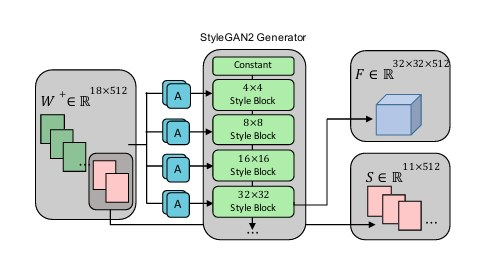
\includegraphics[width=0.6\textwidth]{images/fs_wplus_relation.jpg}
    \caption[ความสัมพันธ์ระหว่าง $FS$ Latent Space และ $W^{+}$ Space]{ความสัมพันธ์ระหว่าง $FS$ Latent Space และ $W^{+}$ Space ใน StyleGAN2 Generator (ดัดแปลงจาก \cite{Zhu_2021})}
    \label{fig:fs_wplus}
\par\vspace{3pt}{\footnotesize\raggedright หมายเหตุ: StyleGAN2 = Style-based Generative Adversarial Network รุ่นที่ 2\par}
\end{figure}

การแปลงภาพกลับเป็นรหัสแฝง (GAN Inversion) มี 2 แนวทาง แนวทางแรกคือแบบปรับค่าซ้ำ (Optimization)
ซึ่งตรึงตัวสร้างไว้ แล้วปรับรหัสด้วยการลดค่าตามเกรเดียนต์ (Gradient Descent) ซ้ำหลายร้อยรอบ
เกรเดียนต์ (Gradient) คือทิศทางที่บอกว่าควรปรับค่าไปทางใดเพื่อให้ค่าสูญเสียลดลง วิธีนี้แม่นยำแต่ช้า
ตัวอย่างคือวิธี Improved Image2StyleGAN (II2S)~\cite{zhu2021improvedstyleganembeddinggood} ที่ Barbershop ใช้
แนวทางที่สองคือแบบตัวเข้ารหัส (Encoder) ซึ่งฝึกเครือข่ายให้คำนวณรหัสของภาพได้ในการคำนวณรอบเดียว
วิธีนี้เร็ว ตัวอย่างคือ Encoder for Editing (E4E)~\cite{tov2021designingencoderstyleganimage} และ FS Encoder ที่ HairFastGAN ใช้
ภาพที่~\ref{fig:fs_recon} เปรียบเทียบภาพจริง (GT) กับภาพที่สร้างคืนจาก $W^{+}$ และจาก $FS$
ภาพในแถวเดียวกันเป็นคนเดียวกัน จะเห็นว่าภาพจาก $W^{+}$ เสียรายละเอียด เช่น ทรงผมและฉากหลัง
ขณะที่ภาพจาก $FS$ ใกล้กับภาพจริงมาก ซึ่งเป็นเหตุผลที่ทั้งสองโมเดลเลือกทำงานในพื้นที่ $FS$

\begin{figure}[H]
    \centering
    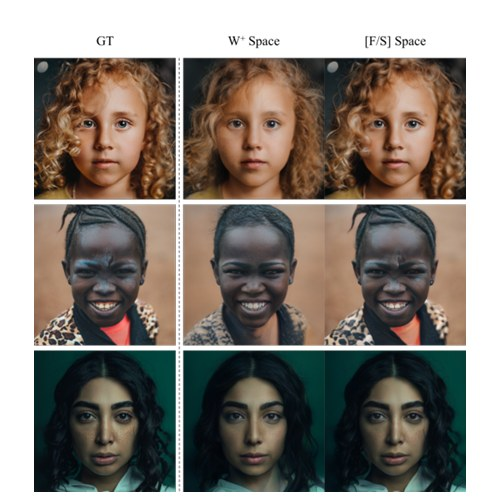
\includegraphics[width=0.55\textwidth]{images/fs_wplus_reconstruction.jpg}
    \caption[เปรียบเทียบคุณภาพการสร้างภาพคืนระหว่าง $W^{+}$ และ $FS$]{เปรียบเทียบคุณภาพการสร้างภาพคืน (Reconstruction) ระหว่างภาพจริง (GT), $W^{+}$ Space และ $FS$ Space (จาก \cite{Zhu_2021})}
    \label{fig:fs_recon}
\end{figure}

% -----------------------------------------------------------
\subsection{การทำงานของโมเดล HairFastGAN}
\label{sec:hairfastgan}
% -----------------------------------------------------------
HairFastGAN~\cite{nikolaev2024hairfastganrealisticrobusthair} รับภาพ 3 ภาพ ได้แก่ ภาพใบหน้าของผู้ใช้ (Source Image)
ภาพที่มีทรงผมที่ต้องการ (Shape Image) และภาพที่มีสีผมที่ต้องการ (Color Image)
แล้วสร้างภาพที่ยังเป็นใบหน้าของผู้ใช้ แต่ทรงผมและสีผมเปลี่ยนตามภาพอ้างอิง
ทุกขั้นทำบนพื้นที่ $FS$ ที่อธิบายในหัวข้อที่~\ref{sec:stylegan2} โดย $F$ (ขนาด $32 \times 32$) บอกรูปร่างของผมและกรอบหน้า
และ $S$ บอกสีและพื้นผิว เพราะสองส่วนนี้แยกกัน จึงเปลี่ยนทรงหรือสีผมได้โดยไม่กระทบใบหน้า

ภาพที่~\ref{fig:hairfastgan_pipeline} แสดงภาพรวมของ HairFastGAN
ข้อมูลไหลจากซ้ายไปขวา ภาพทั้ง 3 ภาพถูกเข้ารหัสก่อน
แล้วผ่านโมดูลจัดแนว 4 โมดูลตามลำดับ ได้แก่ การปรับท่าทาง (Pose Alignment กรอบสีแดง)
การถ่ายโอนรูปทรง (Shape Alignment กรอบสีฟ้า) การถ่ายโอนสี (Color Alignment กรอบสีม่วง)
และการปรับรายละเอียด (Refinement Alignment กรอบสีเหลือง)
ภาพย่อยในแต่ละกรอบแสดงหน้ากากและภาพกลางที่เกิดขึ้นในขั้นนั้น

\begin{figure}[H]
    \centering
    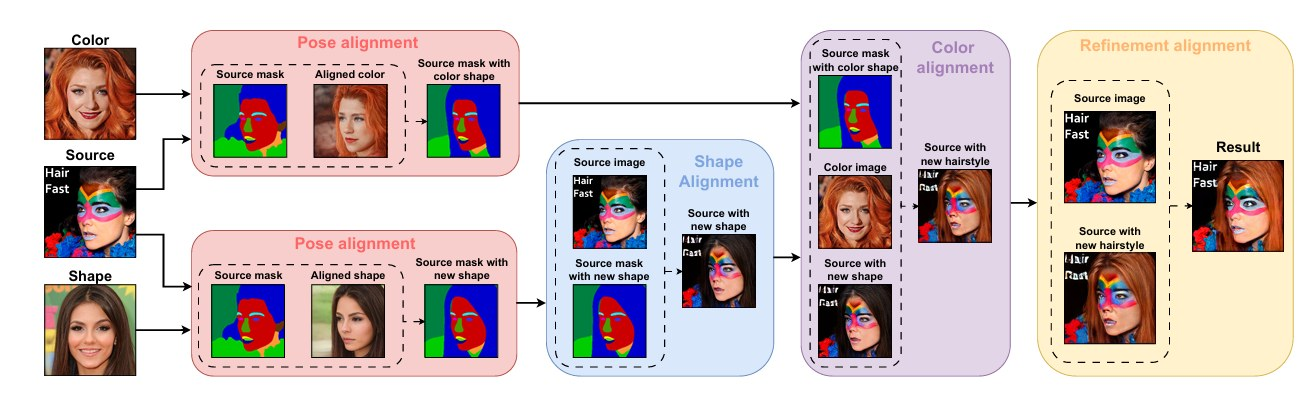
\includegraphics[width=\textwidth]{images/hfg_overview.jpg}
    \caption[ภาพรวมขั้นตอนการทำงานของโมเดล HairFastGAN]{ภาพรวมสถาปัตยกรรมและกระบวนการทำงานของโมเดล HairFastGAN ผ่านโมดูล Pose, Shape, Color และ Refinement Alignment (จาก \cite{nikolaev2024hairfastganrealisticrobusthair})}
    \label{fig:hairfastgan_pipeline}
\end{figure}

\subsubsection{Pose Alignment (การปรับท่าทาง)}
ถ้าคนในภาพทรงผมหันไปคนละทางกับคนในภาพใบหน้า ผมจะถูกวางผิดตำแหน่ง
โมดูลนี้จึงใช้ Rotate Encoder คำนวณรหัสชุดใหม่ของภาพทรงผมให้หันไปทางเดียวกับภาพใบหน้า
ตามสมการที่~(\ref{eq:rotate_enc})
รหัสที่ใช้ในขั้นนี้มาจาก E4E ซึ่งละเอียดพอสำหรับการสร้างหน้ากาก เพราะขั้นนี้ยังไม่ต้องใช้รายละเอียดของเส้นผม
Rotate Encoder แก้เฉพาะรหัส 6 ลำดับแรกของ $W^{+}$ ซึ่งควบคุมลักษณะทางเรขาคณิต เช่น มุมที่ศีรษะหัน
และไม่แตะรหัสอีก 12 ลำดับที่เหลือ จึงหมุนท่าทางได้โดยไม่เปลี่ยนทรงผม
ในงานต้นฉบับ ภาพสีผมก็ผ่านขั้นนี้ด้วย
เพื่อหาหน้ากากผมของภาพสีผมที่หันตามใบหน้า สำหรับใช้ต่อในโมดูลสี
\begin{equation}
    w^{1:6}_\text{rotate} = \text{RotateEnc}\!\left(w^{1:6}_\text{source},\; w^{1:6}_\text{shape}\right)
    \label{eq:rotate_enc}
\end{equation}
\begin{vardef}
$w^{1:6}_\text{rotate}$ & รหัสในพื้นที่ $W^{+}$ 6 ลำดับแรกของภาพทรงผมที่ถูกหมุนให้หันตามใบหน้าแล้ว \\
$\text{RotateEnc}$ & เครือข่ายหมุนรหัส (Rotate Encoder) \\
$w^{1:6}_\text{source}$ & รหัส 6 ลำดับแรกของภาพใบหน้าต้นฉบับ (เก็บท่าทางเป้าหมาย) \\
$w^{1:6}_\text{shape}$ & รหัส 6 ลำดับแรกของภาพอ้างอิงทรงผม
\end{vardef}
จากนั้นนำรหัสที่หมุนแล้วไปวาดเป็นภาพ แล้วให้ BiSeNet (Bilateral Segmentation Network) แบ่งส่วนภาพ
จะได้หน้ากากของภาพอ้างอิงที่หันตามใบหน้า หน้ากากนี้และหน้ากากของภาพใบหน้าจะถูกส่งเข้า Shape Encoder และ Shape Adaptor
เพื่อทำนายหน้ากากของใบหน้าเดิมเมื่อสวมทรงผมใหม่ ตามสมการที่~(\ref{eq:pose_mask})
\begin{equation}
\begin{gathered}
    M_\text{rotate} = \text{BiSeNet}\!\left(G(w_\text{rotate})\right) \\
    M_\text{align} = \text{ShapeAdaptor}\!\left(\text{ShapeEnc}^\text{hair}(M_\text{rotate}),\; \text{ShapeEnc}^\text{face}(M_\text{source})\right)
\end{gathered}
    \label{eq:pose_mask}
\end{equation}
\begin{vardef}
$G$ & ตัวสร้างภาพ StyleGAN2 \\
$w_\text{rotate}$ & รหัสเต็ม 18 ลำดับของภาพอ้างอิง (6 ลำดับแรกที่หมุนแล้ว และ 12 ลำดับเดิม) \\
$M_\text{rotate}$ & หน้ากากของภาพอ้างอิงหลังหมุน \\
$M_\text{source}$ & หน้ากากของภาพใบหน้าต้นฉบับจาก BiSeNet \\
$\text{ShapeEnc}^\text{hair}, \text{ShapeEnc}^\text{face}$ & ตัวเข้ารหัสที่แยกหน้ากากเป็นส่วนผมและส่วนใบหน้า \\
$\text{ShapeAdaptor}$ & เครือข่ายที่รวมสองส่วนกลับเป็นหน้ากากเดียว และเติมบริเวณที่ขาดหาย \\
$M_\text{align}$ & หน้ากากเป้าหมาย คือใบหน้าเดิมที่มีทรงผมใหม่ ($H_\text{align}$ คือส่วนผมของหน้ากากนี้)
\end{vardef}

ผู้พัฒนาฝึก Rotate Encoder ด้วยค่าสูญเสีย 3 ส่วน ได้แก่ การจัดท่าทาง การคงรหัสเดิม
และการรักษาความเหมือนของใบหน้า โดยหารแต่ละส่วนด้วยค่าเฉลี่ยเคลื่อนที่ของส่วนนั้นเอง
เพื่อให้ทั้งสามส่วนมีขนาดใกล้เคียงกัน
\begin{equation}
    \mathcal{L}_\text{Rotate} = \frac{\lambda_\text{pose} \mathcal{L}_\text{pose}}{\text{EMA}_t(\mathcal{L}_\text{pose})} + \frac{\lambda_\text{recon} \mathcal{L}_\text{recon}}{\text{EMA}_t(\mathcal{L}_\text{recon})} + \frac{\lambda_\text{id} \mathcal{L}_\text{id}}{\text{EMA}_t(\mathcal{L}_\text{id})}
    \label{eq:loss_rotate}
\end{equation}
\begin{vardef}
$\mathcal{L}_\text{pose}$ & ค่าสูญเสียจากความต่างของจุดสังเกตบนใบหน้า (Facial Keypoints) 76 จุด \\
$\mathcal{L}_\text{recon}$ & ค่าสูญเสียการคงรหัสเดิม (หมุนไปแล้วหมุนกลับต้องได้รหัสเดิม) \\
$\mathcal{L}_\text{id}$ & ค่าสูญเสียเอกลักษณ์ใบหน้าจาก ArcFace ตามสมการที่~(\ref{eq:arcface_id}) \\
$\lambda_\text{pose}, \lambda_\text{recon}, \lambda_\text{id}$ & น้ำหนักของแต่ละส่วน (6, 2 และ 1 ตามลำดับ) \\
$\text{EMA}_t$ & ค่าเฉลี่ยเคลื่อนที่แบบเอ็กซ์โพเนนเชียล (Exponential Moving Average) ของค่าสูญเสียแต่ละส่วน (ค่าตัวคูณ 0.02)
\end{vardef}
ค่าสูญเสียด้านความเหมือนของใบหน้าคำนวณจากเวกเตอร์ใบหน้าของ ArcFace ตามสมการที่~(\ref{eq:arcface_id})
ถ้า $\mathcal{L}_\text{id}$ มีค่าต่ำ (ค่าโคไซน์สูง) แปลว่าใบหน้ายังเหมือนเดิม
\begin{equation}
    \mathcal{L}_\text{id} = 1 - \cos\!\left(v_\text{output},\; v_\text{source}\right)
    = 1 - \frac{v_\text{output} \cdot v_\text{source}}{\lVert v_\text{output} \rVert \, \lVert v_\text{source} \rVert}
    \label{eq:arcface_id}
\end{equation}
\begin{vardef}
$v_\text{output}$ & เวกเตอร์ใบหน้า 512 มิติจาก ArcFace ของภาพที่สร้างขึ้น \\
$v_\text{source}$ & เวกเตอร์ใบหน้าของภาพต้นฉบับ \\
$\cos(\cdot,\cdot)$ & ความคล้ายโคไซน์ (Cosine Similarity) มีค่า $-1$ ถึง 1 โดย 1 คือเหมือนที่สุด
\end{vardef}

ภาพที่~\ref{fig:ex_pose} แสดงตัวอย่างการทำงานของโมดูลนี้
แถวบนคือการหมุนหน้ากากของภาพสีผม (ใช้ในขั้นสี) และแถวล่างคือการหมุนภาพทรงผม
ภาพ ``Source mask'' คือหน้ากากของใบหน้าต้นฉบับ ภาพ ``Aligned shape'' คือภาพทรงผมที่หมุนแล้ว
และภาพขวาสุดคือหน้ากากใหม่ที่ผมหันตรงกับใบหน้าต้นฉบับ

\begin{figure}[H]
    \centering
    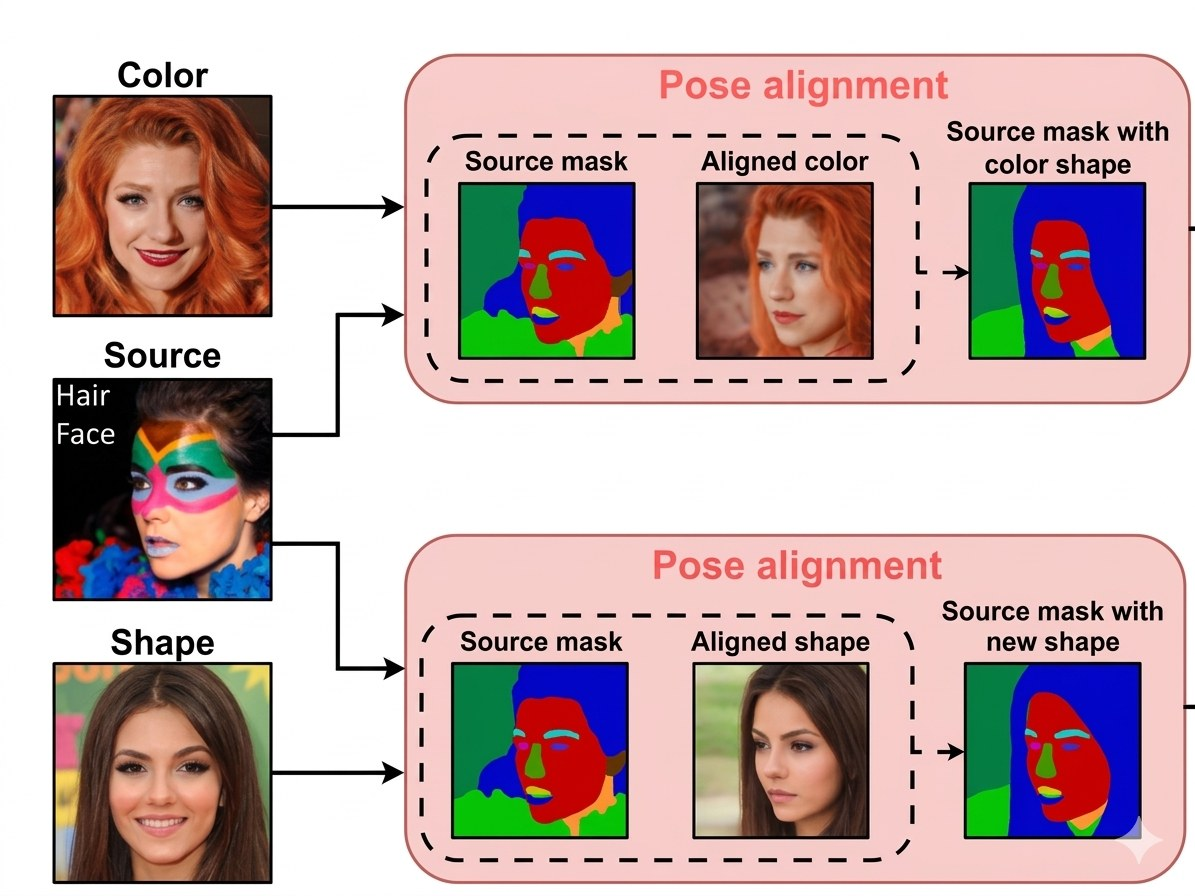
\includegraphics[width=0.6\textwidth]{images/example_pose_alignment.jpg}
    \caption[ตัวอย่างการทำงานของ Pose Alignment]{ตัวอย่างการทำงานของ Pose Alignment ที่ปรับ Mask ผมของภาพอ้างอิงให้หันตามใบหน้าต้นฉบับ (จาก \cite{nikolaev2024hairfastganrealisticrobusthair})}
    \label{fig:ex_pose}
\end{figure}

\subsubsection{Shape Alignment (การถ่ายโอนรูปทรงผม)}
โมดูลนี้นำทรงผมใหม่มาวางบนโครงหน้าเดิม แต่ก่อนย้ายทรงผมต้องแก้ปัญหาหนึ่งก่อน
คือ $F$ ที่ได้จาก FS Encoder สร้างภาพคืนได้แม่นยำมาก แต่เก็บรายละเอียดของผมไว้แน่นจนเปลี่ยนสีผมผ่าน $S$ ได้ยาก
ผู้พัฒนาจึงเข้ารหัสภาพเดียวกันด้วย E4E อีกทางหนึ่ง ซึ่งสร้างภาพคืนได้หยาบกว่าแต่แก้ไขได้ง่ายกว่า
แล้วผสม $F$ ทั้งสองแบบเฉพาะบริเวณผม (FS and $W^{+}$ Mixing) ตามสมการที่~(\ref{eq:hfg_mix})
\begin{equation}
    F^\text{mix}_{32} = \bar{H} \cdot F^\text{FSE}_{32} + (1 - \alpha) \cdot H \cdot F^\text{FSE}_{32} + \alpha \cdot H \cdot F^\text{E4E}_{32}
    \label{eq:hfg_mix}
\end{equation}
\begin{vardef}
$F^\text{mix}_{32}$ & แผนที่คุณลักษณะขนาด $32 \times 32$ หลังผสม \\
$F^\text{FSE}_{32}, F^\text{E4E}_{32}$ & แผนที่คุณลักษณะที่ได้จาก FS Encoder และจาก E4E \\
$H, \bar{H}$ & หน้ากากผมจาก BiSeNet ที่ย่อเหลือ $32 \times 32$ และส่วนกลับ ($\bar{H} = 1 - H$) \\
$\alpha$ & สัดส่วนการผสม ผู้พัฒนาและงานวิจัยนี้ใช้ 0.95
\end{vardef}
ค่า $\alpha = 0.95$ หมายความว่าบริเวณผมใช้ $F$ จาก E4E ร้อยละ 95 และจาก FS Encoder เพียงร้อยละ 5
ส่วนใบหน้าและพื้นหลังยังใช้ $F$ จาก FS Encoder ทั้งหมด จึงเก็บรายละเอียดของใบหน้าไว้ได้ครบ

ขั้นต่อมาคือเติมส่วนที่ขาดหาย (Inpainting) เช่น หน้าผากที่เคยถูกผมบังแต่ทรงใหม่เปิดออก
ผู้พัฒนาใช้ SEAN (Semantic Region-Adaptive Normalization)~\cite{Zhu_2020}
ซึ่งเข้ารหัสสไตล์ของแต่ละบริเวณในภาพ แล้ววาดภาพใหม่ขนาด $256 \times 256$ ตามหน้ากาก $M_\text{align}$
จากนั้นเข้ารหัสภาพที่ได้ด้วย E4E อีกครั้งเป็น $F^\text{inpaint}$
เพราะ E4E ช่วยลบสิ่งแปลกปลอมที่ SEAN อาจสร้างขึ้น เช่น ใบหูที่ผิดรูป
ขั้นตอนทั้งหมดนี้ทำกับทั้งภาพต้นฉบับและภาพทรงผม
สุดท้ายจึงเลือก $F$ จาก 4 แหล่งตามหน้ากาก ดังสมการที่~(\ref{eq:shape_combine})
\begin{equation}
\begin{aligned}
    F^{\text{align}}_{32} = & \; H_\text{align} \cdot H_\text{shape} \cdot F^{\text{mix}}_\text{shape}
    + H_\text{align} \cdot \bar{H}_\text{shape} \cdot F^{\text{inpaint}}_\text{shape} \\
    & + \bar{H}_\text{align} \cdot \bar{H}_\text{source} \cdot F^{\text{mix}}_\text{source}
    + \bar{H}_\text{align} \cdot H_\text{source} \cdot F^{\text{inpaint}}_\text{source}
\end{aligned}
\label{eq:shape_combine}
\end{equation}
\begin{vardef}
$F^{\text{align}}_{32}$ & แผนที่คุณลักษณะขนาด $32 \times 32$ ขั้นสุดท้ายที่จัดทรงผมเข้ากับใบหน้าแล้ว \\
$H_\text{align}$ & หน้ากากทรงผมเป้าหมาย (บริเวณที่ควรมีผมมีค่า 1) และ $\bar{H}_\text{align} = 1 - H_\text{align}$ \\
$H_\text{shape}, H_\text{source}$ & หน้ากากเส้นผมเดิมของภาพอ้างอิงทรงผมและภาพต้นฉบับ (ขีดบนคือส่วนกลับ) \\
$F^{\text{mix}}_\text{shape}, F^{\text{mix}}_\text{source}$ & แผนที่คุณลักษณะหลังผสมตามสมการที่~(\ref{eq:hfg_mix}) ของภาพทรงผมและภาพต้นฉบับ \\
$F^{\text{inpaint}}_\text{shape}, F^{\text{inpaint}}_\text{source}$ & แผนที่คุณลักษณะของภาพที่เติมส่วนที่ขาดหายด้วย SEAN แล้วเข้ารหัสด้วย E4E
\end{vardef}
สมการนี้แบ่งพิกเซลเป็น 4 กรณี ตามว่าพิกเซลนั้นอยู่ในบริเวณผมใหม่หรือไม่ และภาพเดิมมีผมอยู่ตรงนั้นหรือไม่
ถ้าเป็นบริเวณผมใหม่และภาพทรงผมมีผมอยู่ตรงนั้นจริง ก็ใช้ผมจากภาพทรงผมได้ทันที
ถ้าเป็นบริเวณผมใหม่แต่ภาพทรงผมไม่มีผมตรงนั้น (เช่น ภาพทรงผมหันคนละมุม) ต้องใช้ผมที่ SEAN เติมให้
ส่วนบริเวณที่ไม่ใช่ผม ถ้าภาพต้นฉบับไม่เคยมีผมตรงนั้น ก็ใช้ภาพต้นฉบับได้ทันที
แต่ถ้าเคยมีผมบังอยู่ (เช่น ผมหน้าม้าเดิม) ต้องใช้ส่วนที่ SEAN เติมให้แทน

ภาพที่~\ref{fig:hfg_detail1} แสดงโครงสร้างภายในของขั้นนี้
ภาพ (a) คือบล็อกผสมพื้นที่แฝง ซึ่งนำ $F$ จาก FS Encoder และจาก $W^{+}$ มาผสมกันด้วยสัดส่วน $\alpha$
ภาพ (b) แสดงลำดับของโมดูล Pose (สีแดง) ที่ใช้ Rotate Encoder และ BiSeNet
ตามด้วยโมดูล Shape (สีฟ้า) ที่ใช้ตัวเข้ารหัสและตัวถอดรหัสของ SEAN
สร้างทรงผมเป้าหมายบนพื้นที่ $F$ ส่วนภาพที่~\ref{fig:ex_shape} แสดงตัวอย่างผลของขั้นนี้
คือหน้ากากของภาพต้นฉบับที่มีรูปทรงผมใหม่ และภาพต้นฉบับที่สวมทรงผมใหม่แล้ว

\begin{figure}[H]
    \centering
    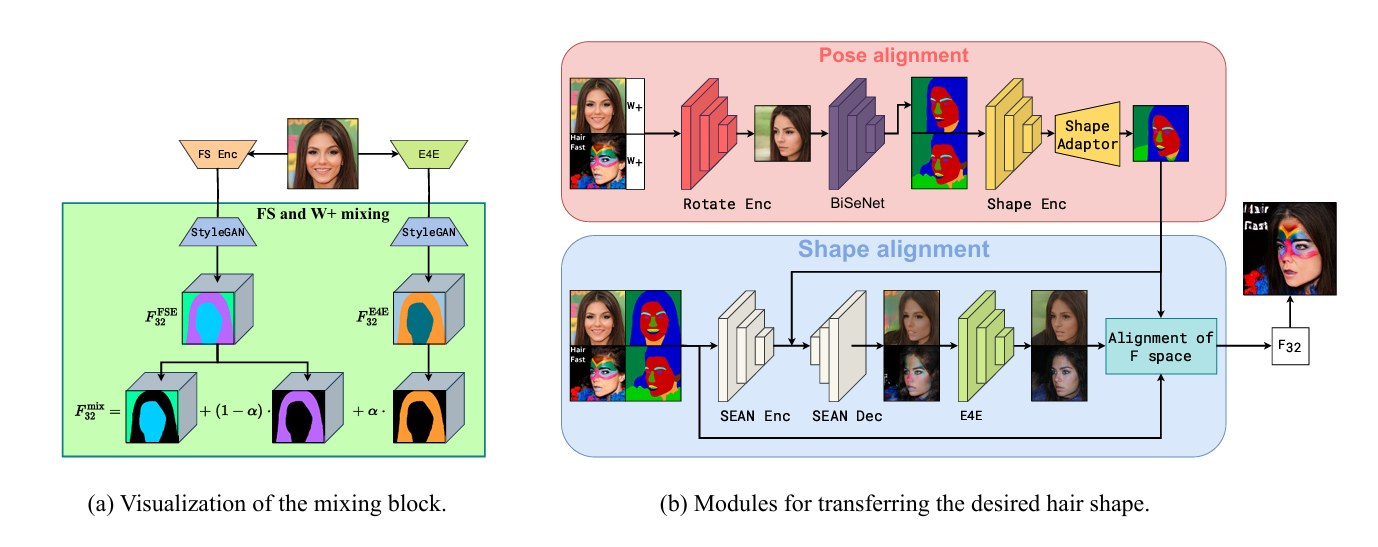
\includegraphics[width=\textwidth]{images/hfg_detail_1.jpg}
    \caption[บล็อกผสมพื้นที่แฝงและโมดูลถ่ายโอนรูปทรงของ HairFastGAN]{(a) บล็อกผสมพื้นที่แฝง $FS$ กับ $W^{+}$ และ (b) โมดูลถ่ายโอนรูปทรงผม (Pose และ Shape Alignment) ของ HairFastGAN (จาก \cite{nikolaev2024hairfastganrealisticrobusthair})}
    \label{fig:hfg_detail1}
\end{figure}

\begin{figure}[H]
    \centering
    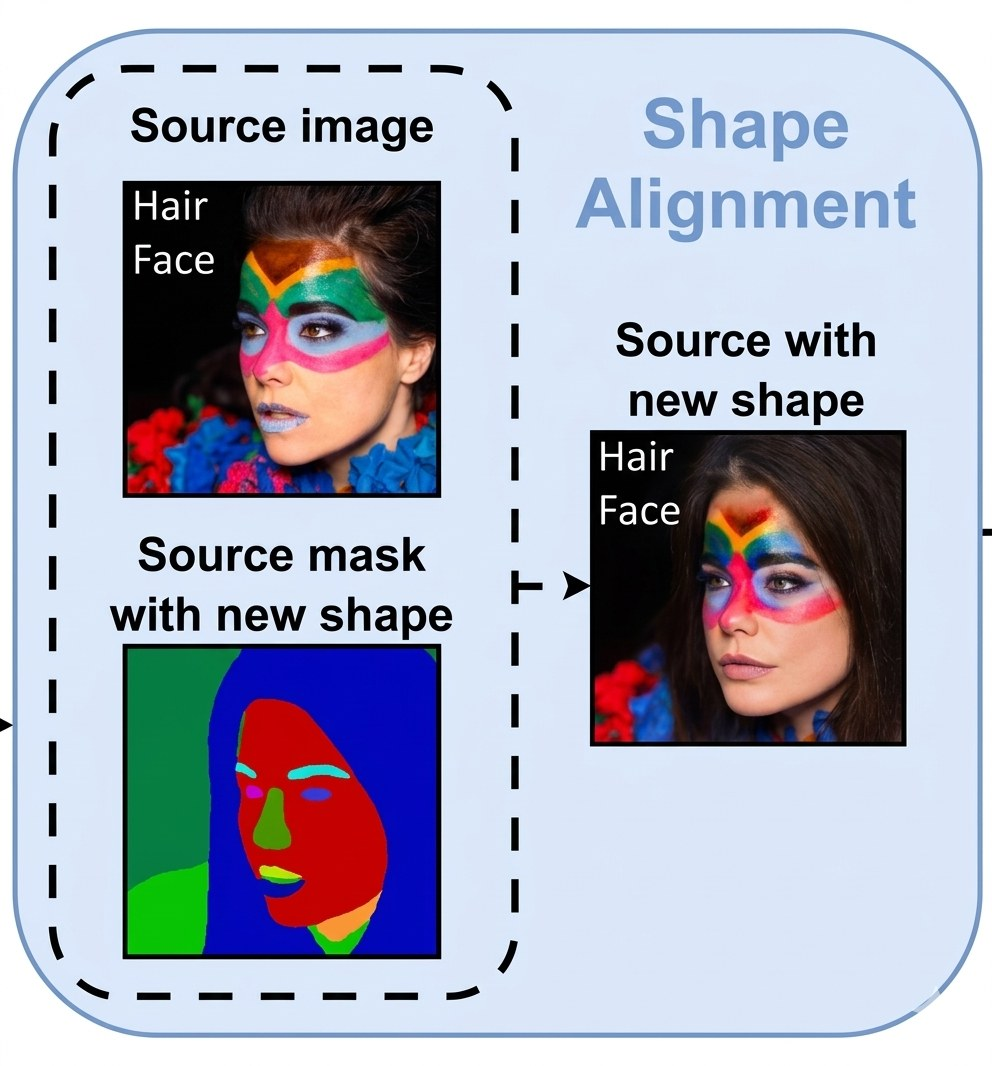
\includegraphics[width=0.45\textwidth]{images/example_shape_alignment.jpg}
    \caption[ตัวอย่างการทำงานของ Shape Alignment]{ตัวอย่างการทำงานของ Shape Alignment ที่สร้างภาพต้นฉบับพร้อมรูปทรงผมใหม่ (จาก \cite{nikolaev2024hairfastganrealisticrobusthair})}
    \label{fig:ex_shape}
\end{figure}

\subsubsection{Color Alignment (การถ่ายโอนสีผม)}
โมดูลนี้เปลี่ยนสีของทรงผมใหม่ให้เป็นสีตามภาพสีผม
ผู้พัฒนาพบว่าการผสม $S$ ของสองภาพด้วยการถัวเฉลี่ยแบบงานก่อนหน้ายังให้สีที่ไม่ดีพอ
จึงสร้างตัวเข้ารหัสผสม (Blending Encoder) ที่ทำนายว่า $S$ ของภาพต้นฉบับต้องเปลี่ยนไปเท่าใด
ภายในประกอบด้วยชั้นปรับค่า (Modulation) 5 บล็อก ซึ่งรับ $S$ ของภาพสีผมและเวกเตอร์จาก CLIP
(Contrastive Language-Image Pre-training) มาคำนวณค่าสเกลและค่าเลื่อน ดังสมการที่~(\ref{eq:s_blend})
โดย $\text{emb}_\text{face}$ คือเวกเตอร์ของภาพต้นฉบับที่ลบผมออกแล้ว
และ $\text{emb}_\text{hair}$ คือเวกเตอร์ของภาพสีผมที่เหลือแต่ผม
จากนั้นวาดภาพด้วย $F^\text{align}_{32}$ จากโมดูล Shape และ $S_\text{blend}$ จะได้ภาพ $I_\text{blend}$
\begin{equation}
    S_\text{blend} = \text{BlendEnc}\!\left(S_\text{source},\; S_\text{color},\; \text{emb}_\text{face},\; \text{emb}_\text{hair}\right)
    \label{eq:s_blend}
\end{equation}
\begin{vardef}
$S_\text{blend}$ & รหัสสไตล์ชุดใหม่ที่มีสีผมตามภาพอ้างอิง \\
$\text{BlendEnc}$ & ตัวเข้ารหัสผสม (Blending Encoder) \\
$S_\text{source}, S_\text{color}$ & รหัสสไตล์ของภาพใบหน้าต้นฉบับและภาพอ้างอิงสีผม \\
$\text{emb}_\text{face}, \text{emb}_\text{hair}$ & เวกเตอร์ความหมายจาก CLIP ของบริเวณใบหน้าและบริเวณผม
\end{vardef}
ผู้พัฒนาฝึกโมดูลนี้ด้วยค่าสูญเสียที่วัดความคล้ายเชิงความหมายผ่าน CLIP
แทนการวัดความต่างทีละพิกเซล ตามสมการที่~(\ref{eq:loss_colormodule})
ส่วนแรกบังคับให้ผมมีสีเหมือนภาพสีผม และส่วนที่สองบังคับให้ใบหน้ายังเหมือนภาพต้นฉบับ
\begin{equation}
    \begin{aligned}
    \mathcal{L}_\text{ColorModule} = \; & \lambda_\text{color} \mathcal{L}_\text{CLIP}\!\left(I_\text{blend}, I_\text{color}, H_\text{align}, H_\text{color}\right) \\
    & + \lambda_\text{face} \mathcal{L}_\text{CLIP}\!\left(I_\text{blend}, I_\text{source}, M_\text{target}, M_\text{target}\right)
    \end{aligned}
    \label{eq:loss_colormodule}
\end{equation}
\begin{vardef}
$\mathcal{L}_\text{CLIP}$ & ค่าสูญเสีย $1 -$ ความคล้ายโคไซน์ของคุณลักษณะจาก CLIP เฉพาะบริเวณที่กำหนด \\
$I_\text{blend}$ & ภาพที่สร้างหลังเปลี่ยนสีผม \\
$I_\text{color}, I_\text{source}$ & ภาพอ้างอิงสีผมและภาพใบหน้าต้นฉบับ \\
$H_\text{align}, H_\text{color}$ & หน้ากากผมของภาพผลลัพธ์และของภาพอ้างอิงสีผม \\
$M_\text{target}$ & หน้ากากบริเวณที่ไม่ใช่ผมทั้งในภาพต้นฉบับและในทรงใหม่ ($\bar{H}_\text{source} \cdot \bar{H}_\text{align}$) \\
$\lambda_\text{color}, \lambda_\text{face}$ & น้ำหนักของส่วนสีผมและส่วนใบหน้า (ผู้พัฒนาใช้ 1 ทั้งคู่)
\end{vardef}

\subsubsection{Refinement Alignment (การฟื้นฟูรายละเอียด)}
แม้สีผมจะถูกต้องแล้ว แต่ภาพ $I_\text{blend}$ ผ่านการเข้ารหัสมาหลายครั้ง
รายละเอียดของใบหน้าและพื้นหลังจึงหายไปบางส่วน และสีผิวอาจเพี้ยนจากเดิม
โมดูลนี้ (ในโค้ดเรียกว่า PostProcess) จึงเข้ารหัสทั้ง $I_\text{blend}$ และภาพต้นฉบับใหม่
ด้วย FS Encoder ตัวใหญ่ที่ให้ $F$ ขนาด $64 \times 64$ ซึ่งละเอียดกว่าขั้นก่อน 4 เท่า
แล้วใช้ตัวผสม Fused $F$ และ Fused $S$ Encoder รวมสองภาพเข้าด้วยกัน
ให้ได้ทั้งผมใหม่จาก $I_\text{blend}$ และรายละเอียดใบหน้าจากภาพต้นฉบับ
ก่อนส่งให้ StyleGAN2 วาดภาพสุดท้าย ดังสมการที่~(\ref{eq:i_final})
\begin{equation}
    I_\text{final} = \text{StyleGAN}\!\left(\text{FusedFEnc}(F^{\text{blend}}_{64}, F^{\text{source}}_{64}),\; S_\text{final}\right)
    \label{eq:i_final}
\end{equation}
\begin{vardef}
$I_\text{final}$ & ภาพผลลัพธ์สุดท้ายของ HairFastGAN \\
$\text{FusedFEnc}$ & ตัวเข้ารหัสที่ผสมแผนที่คุณลักษณะของสองภาพ \\
$F^{\text{blend}}_{64}$ & แผนที่คุณลักษณะขนาด $64 \times 64$ ของภาพหลังเปลี่ยนทรงและสีผม \\
$F^{\text{source}}_{64}$ & แผนที่คุณลักษณะขนาด $64 \times 64$ ของภาพใบหน้าต้นฉบับ \\
$S_\text{final}$ & รหัสสไตล์สุดท้าย เท่ากับรหัสเฉลี่ยของ StyleGAN2 บวกผลจากตัวเข้ารหัส Fused $S$ ที่รับ $S$ ของสองภาพ \\
$\text{StyleGAN}$ & ตัวสร้างภาพ StyleGAN2 ที่ตรึงไว้
\end{vardef}
โมดูลนี้ถูกฝึกด้วยค่าสูญเสียหลายส่วน ซึ่งเขียนแบบย่อได้ดังสมการที่~(\ref{eq:loss_refine})
ในงานต้นฉบับ แต่ละส่วนคำนวณกับภาพหลายคู่ เช่น เทียบใบหน้าของผลลัพธ์กับภาพต้นฉบับ
และเทียบผมของผลลัพธ์กับ $I_\text{blend}$ โดยคูณหน้ากากก่อนเทียบ
\begin{equation}
    \mathcal{L}_\text{Refine} = \lambda_\text{id}\mathcal{L}_\text{id} + \lambda_\text{m-LPIPS}\mathcal{L}_\text{m-LPIPS} + \lambda_\text{feat}\mathcal{L}_\text{feat} + \lambda_\text{DSC++}\mathcal{L}_\text{DSC++} + \lambda_\text{inpaint}\mathcal{L}_\text{inpaint} + \lambda_\text{ADV}\mathcal{L}_\text{ADV}
    \label{eq:loss_refine}
\end{equation}
\begin{vardef}
$\mathcal{L}_\text{id}$ & ค่าสูญเสียเอกลักษณ์ใบหน้าจาก ArcFace ตามสมการที่~(\ref{eq:arcface_id}) \\
$\mathcal{L}_\text{m-LPIPS}$ & ค่าความต่างเชิงการรับรู้แบบหลายสเกล (Multi-scale LPIPS) ที่ผู้พัฒนา FS Encoder เสนอ \\
$\mathcal{L}_\text{feat}$ & ค่าความต่างกำลังสองระหว่าง $F$ ที่ได้กับ $F$ ที่วาดจาก $S$ ช่วยให้การฝึกช่วงแรกนิ่ง \\
$\mathcal{L}_\text{DSC++}$ & ค่าสูญเสียไดซ์แบบปรับเทียบ (DSC++)~\cite{yeung2022calibratingdicelosshandle} ที่บังคับให้หน้ากากผมของผลลัพธ์ตรงกับของ $I_\text{blend}$ \\
$\mathcal{L}_\text{inpaint}$ & ค่า m-LPIPS เฉพาะบริเวณที่ต้องเติมใหม่ ช่วยให้ส่วนที่เติมกลืนกับภาพ \\
$\mathcal{L}_\text{ADV}$ & ค่าสูญเสียปรปักษ์ (Adversarial Loss) จากตัวจำแนกของ StyleGAN2 เพื่อให้ภาพสมจริง \\
$\lambda$ & น้ำหนักของแต่ละส่วน ผู้พัฒนาใช้ $\lambda_\text{id} = 0.1$, $\lambda_\text{m-LPIPS} = 0.4$, $\lambda_\text{feat} = 0.01$, $\lambda_\text{DSC++} = 0.1$, $\lambda_\text{inpaint} = 0.2$ และ $\lambda_\text{ADV} = 0.2$
\end{vardef}

ภาพที่~\ref{fig:hfg_detail2} แสดงโครงสร้างของสองโมดูลสุดท้าย
ภาพ (a) แสดงโมดูลสีที่นำภาพสีผมเข้า CLIP แล้วส่งเวกเตอร์ไปยังชั้นปรับค่า (Modulation)
เพื่อเปลี่ยนรหัสสไตล์ ภาพ (b) แสดงโมดูลปรับรายละเอียดที่รับทั้งภาพหลังเปลี่ยนสีและภาพต้นฉบับ
แล้วผสมคุณลักษณะผ่าน Fused $F$ และ Fused $S$ Encoder ก่อนส่งเข้า StyleGAN2
ส่วนภาพที่~\ref{fig:ex_color_refine} แสดงตัวอย่างผล (a) คือภาพที่ได้สีผมจากภาพสีผมแล้ว
และ (b) คือภาพผลลัพธ์สุดท้ายที่ได้จากการผสมภาพต้นฉบับกับภาพที่มีทรงและสีใหม่

\begin{figure}[H]
    \centering
    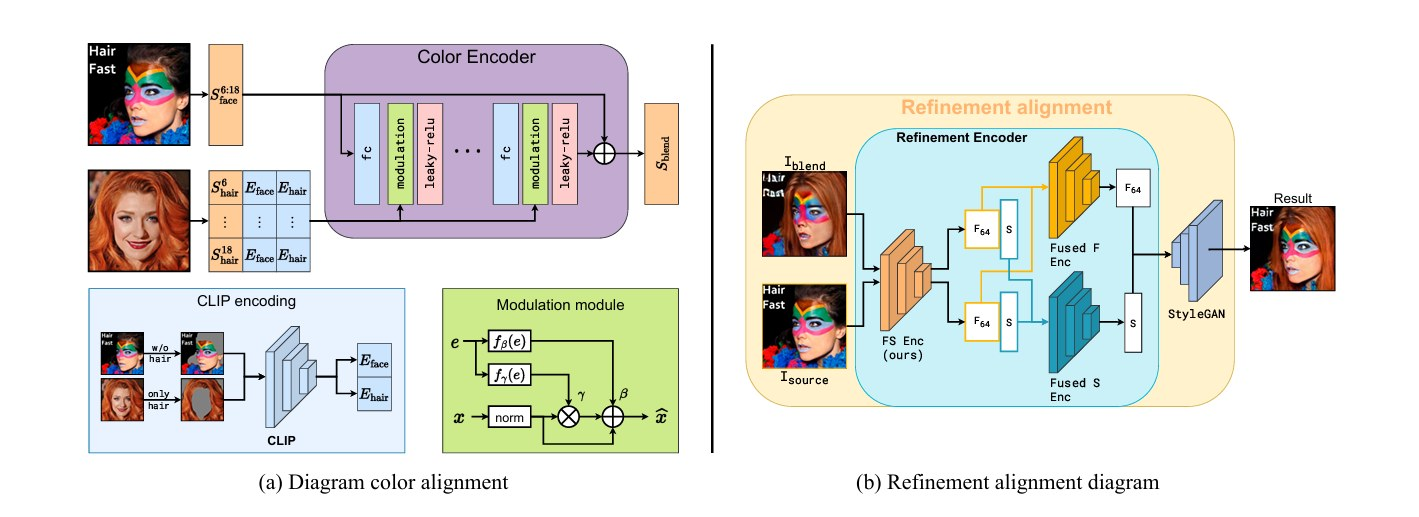
\includegraphics[width=\textwidth]{images/hfg_detail_2.jpg}
    \caption[โครงสร้างโมดูล Color และ Refinement ของ HairFastGAN]{(a) โครงสร้างโมดูล Color Alignment และ (b) โมดูล Refinement Alignment ของ HairFastGAN (จาก \cite{nikolaev2024hairfastganrealisticrobusthair})}
    \label{fig:hfg_detail2}
\end{figure}

\begin{figure}[H]
    \centering
    \begin{subfigure}{0.33\textwidth}
    \centering
    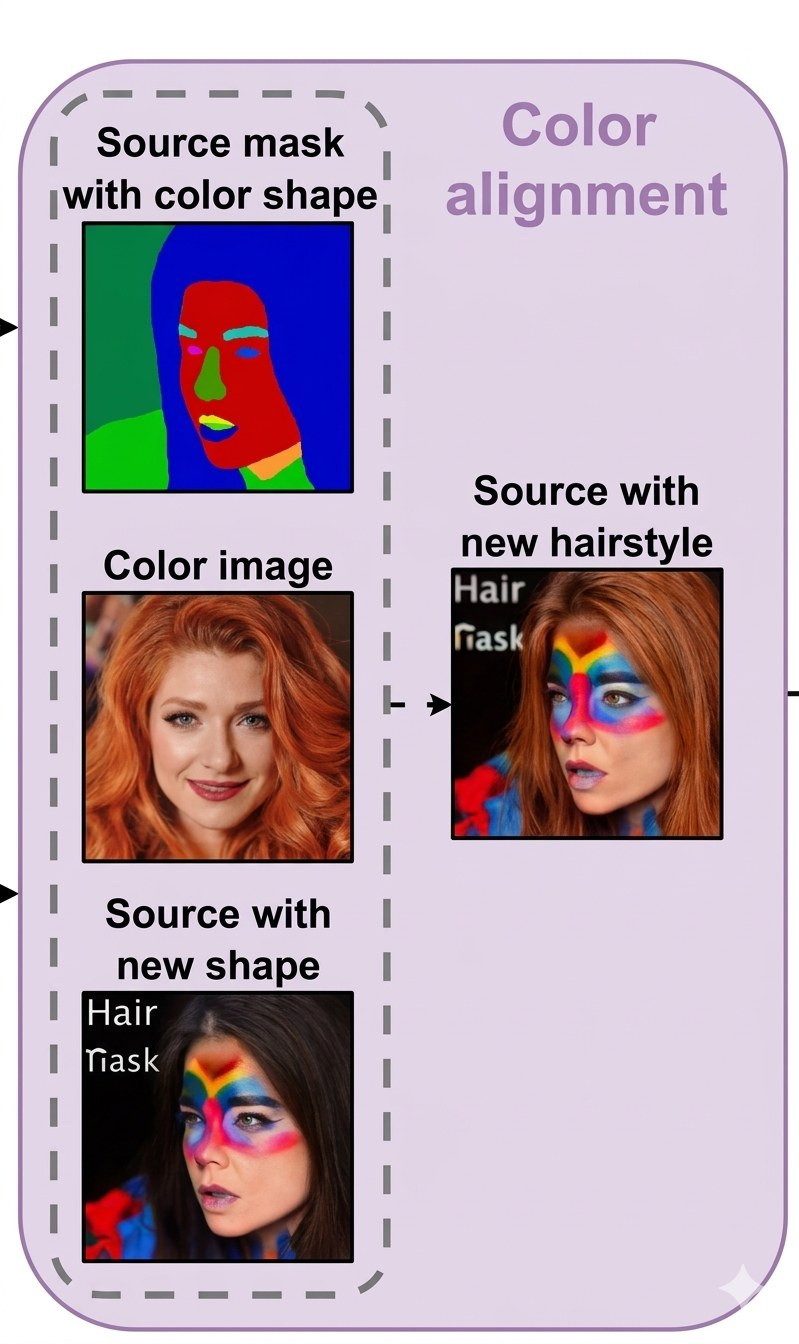
\includegraphics[width=\textwidth]{images/example_Color_alignment.jpg}
    \caption{Color Alignment}
    \end{subfigure}
    \hspace{1em}
    \begin{subfigure}{0.37\textwidth}
    \centering
    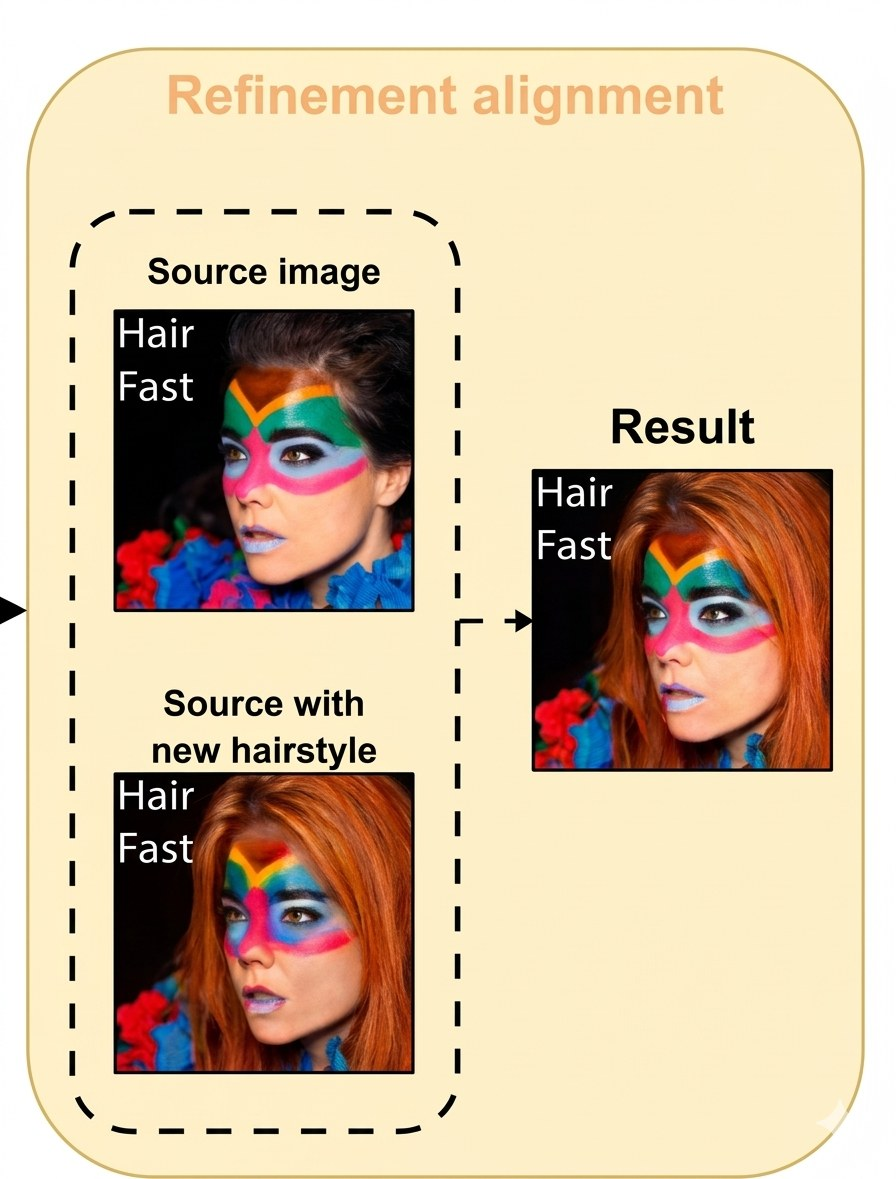
\includegraphics[width=\textwidth]{images/example_Refinement_alignment.jpg}
    \caption{Refinement Alignment}
    \end{subfigure}
    \caption[ตัวอย่างการทำงานของ Color และ Refinement Alignment]{ตัวอย่างการทำงานของโมดูล Color และ Refinement Alignment (จาก \cite{nikolaev2024hairfastganrealisticrobusthair})}
    \label{fig:ex_color_refine}
\end{figure}

เมื่อเข้าใจหน้าที่ของแต่ละโมดูลแล้ว ผู้วิจัยจึงย้อนกลับไปดูปัญหาที่พบจากการรันโมเดลตั้งต้น
สีผมที่เป็นปื้นเกิดจากโมดูล Color ส่วนใบหน้าที่ซีดเกิดจากโมดูล Refinement
ที่ดึงรายละเอียดของภาพต้นฉบับกลับมาได้ไม่ครบ ขณะที่ทรงผมและท่าทางส่วนใหญ่ออกมาถูกต้องอยู่แล้ว
ผู้วิจัยจึงล็อกโมดูล Embedding, Pose และ Shape ไว้ คือไม่ปรับน้ำหนักของโมดูลเหล่านี้
และปรับจูนเฉพาะโมดูล Color (ชั้น Modulation ของ Blending Encoder)
กับโมดูล Refinement ทั้งโมดูล (PostProcess ซึ่งประกอบด้วย FS Encoder ตัวใหญ่และตัวผสม Fused $F$/$S$)
โดยใช้ฟังก์ชันความสูญเสียที่ผู้วิจัยออกแบบเองแทนฟังก์ชันเดิมของผู้พัฒนา
(รายละเอียดในหัวข้อที่~\ref{sec:pipe_hfg} และ~\ref{sec:loss})

% -----------------------------------------------------------
\subsection{การทำงานของโมเดล Barbershop}
\label{sec:barbershop}
% -----------------------------------------------------------
Barbershop~\cite{Zhu_2021} ไม่ได้ฝึกเครือข่ายให้คำนวณรหัสเหมือน HairFastGAN
แต่ค้นหารหัสที่ดีที่สุดด้วยการปรับค่าซ้ำไปเรื่อย ๆ หลายร้อยรอบ (Iterative Optimization)
คล้ายการค่อย ๆ หมุนปุ่มจนภาพที่ได้ตรงที่สุด วิธีนี้ช้า แต่ได้รหัสที่เหมาะกับภาพนั้นจริง ๆ
จึงเก็บรายละเอียดเฉพาะของแต่ละคน เช่น ไฝหรือริ้วรอย ได้ดี และทำงานบนพื้นที่ $FS$ เหมือน HairFastGAN
ข้อเสียคือต้องค้นหารหัสแฝง (Latent) ใหม่ทุกภาพ ยิ่งตั้งให้ค้นหานาน ผลลัพธ์ก็ยิ่งดีขึ้น แต่ก็ยิ่งช้า

ภาพที่~\ref{fig:barbershop_pipeline} แสดงขั้นตอนของ Barbershop จากซ้ายไปขวา
ภาพนำเข้า (a)--(b) ถูกเข้ารหัสเป็น $C^\text{rec}$ จากนั้นสร้างหน้ากากเป้าหมาย $M$ (c)
แล้วปรับรหัสของแต่ละภาพให้ตรงกับ $M$ ได้ $W^\text{align}$ และ $C^\text{align}$ (d)--(g)
จากนั้นผสมโครงสร้างเป็น $F^\text{blend}$ (h) และผสมสไตล์เป็น $S^\text{blend}$
ก่อนรวมเป็น $C^\text{blend}$ (i) ที่ใช้วาดภาพผลลัพธ์

\begin{figure}[H]
    \centering
    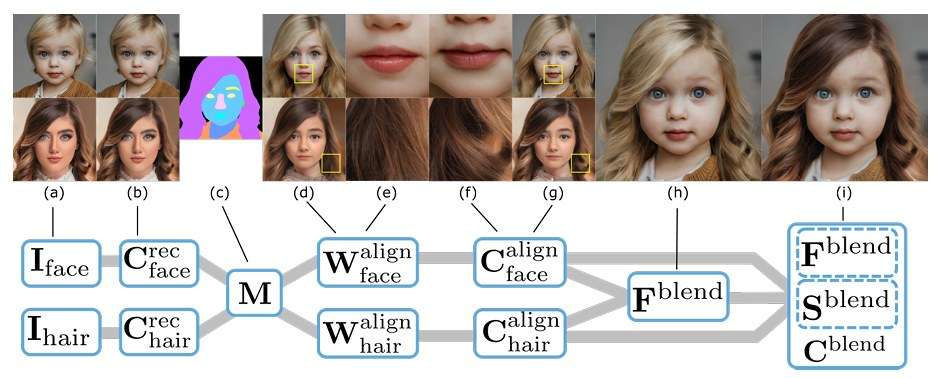
\includegraphics[width=\textwidth]{images/bs_overview.jpg}
    \caption[ภาพรวมกระบวนการทำงานของโมเดล Barbershop]{สถาปัตยกรรมและอัลกอริทึมการทำงานของโมเดล Barbershop ในพื้นที่ $FS$ Latent Space (จาก \cite{Zhu_2021})}
    \label{fig:barbershop_pipeline}
\end{figure}

\subsubsection{FS Latent Space Embedding (การค้นหารหัสของภาพ)}
ขั้นแรกคือค้นหารหัสแฝง $C = (F, S)$ ที่เมื่อส่งเข้า StyleGAN2 แล้วได้ภาพใกล้กับภาพนำเข้าแต่ละภาพมากที่สุด
ด้วยการลดค่าตามเกรเดียนต์ซ้ำหลายรอบ ตามสมการที่~(\ref{eq:barbershop_opt})
\begin{equation}
    C^\text{rec}_k = \arg\min_{C}\; \left( \mathcal{L}_\text{LPIPS}(G(C),\; I_k) + \mathcal{L}_F(F) \right)
    \label{eq:barbershop_opt}
\end{equation}
\begin{vardef}
$C^\text{rec}_k$ & รหัสแฝงที่ดีที่สุดของภาพที่ $k$ \\
$G(C)$ & ภาพที่ StyleGAN2 วาดจากรหัส $C$ \\
$I_k$ & ภาพนำเข้าภาพที่ $k$ (ภาพใบหน้า ภาพทรงผม หรือภาพสีผม) \\
$\mathcal{L}_\text{LPIPS}$ & ค่าความต่างเชิงการรับรู้ (Learned Perceptual Image Patch Similarity)~\cite{zhang2018unreasonableeffectivenessdeepfeatures} ที่วัดจากคุณลักษณะของเครือข่าย VGG (Visual Geometry Group)~\cite{simonyan2015deepconvolutionalnetworkslargescale} \\
$\mathcal{L}_F(F)$ & ค่าสูญเสียที่ไม่ให้ $F$ ห่างจากค่าเริ่มต้น เท่ากับ $\lVert F - F^\text{init}_k \rVert^2$
\end{vardef}

\subsubsection{Aligned Embedding (การปรับโครงสร้างให้ตรงหน้ากาก)}
ขั้นนี้บังคับให้รหัสแฝงสร้างภาพที่มีผมอยู่ตามหน้ากากเป้าหมาย $M$
ภาพที่~\ref{fig:target_mask} แสดงวิธีสร้าง $M$ จากหน้ากากของแต่ละภาพ
หน้ากาก $M_1$, $M_2$ และ $M_3$ คือแผนที่ส่วนภาพของภาพนำเข้าแต่ละภาพ
ลูกศรสีแดงแสดงว่าบริเวณผมนำมาจากภาพทรงผม ส่วนบริเวณใบหน้าและส่วนอื่นนำมาจากภาพใบหน้า
แล้วรวมเป็นหน้ากาก $M$ เพียงหน้ากากเดียว ที่บอกว่าแต่ละพิกเซลของผลลัพธ์ควรเป็นส่วนใด

\begin{figure}[H]
    \centering
    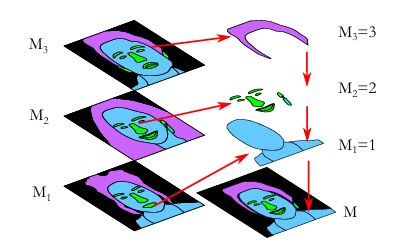
\includegraphics[width=0.5\textwidth]{images/bs_target_mask.jpg}
    \caption[การสร้างหน้ากากเป้าหมายของ Barbershop]{การสร้างหน้ากากเป้าหมาย $M$ จากหน้ากากของภาพแต่ละภาพ ($M_1$, $M_2$, $M_3$) (จาก \cite{Zhu_2021})}
    \label{fig:target_mask}
\end{figure}

การค้นหารหัสที่ตรงกับ $M$ ใช้ค่าสูญเสียตามสมการที่~(\ref{eq:barbershop_align_loss})
\begin{equation}
    w^\text{align}_k = \arg\min_{W}\; \text{XEnt}\!\left(M,\; \text{Segment}(G(W))\right) + \lambda_s \mathcal{L}_s(W)
    \label{eq:barbershop_align_loss}
\end{equation}
\begin{vardef}
$w^\text{align}_k$ & รหัส $W^{+}$ ของภาพที่ $k$ ที่จัดให้ตรงกับหน้ากากแล้ว \\
$\text{XEnt}$ & ค่าสูญเสียครอสเอนโทรปี (Cross-Entropy) ระหว่างหน้ากากเป้าหมายกับผลแบ่งส่วนภาพ \\
$\text{Segment}(G(W))$ & ผลแบ่งส่วนภาพด้วย BiSeNet ของภาพที่วาดจากรหัส $W$ \\
$\mathcal{L}_s(W)$ & ค่าสูญเสียสไตล์เฉพาะบริเวณ (Masked Style Loss) จากเมทริกซ์แกรม \\
$\lambda_s$ & น้ำหนักของค่าสูญเสียสไตล์
\end{vardef}
ขั้นนี้ปรับเฉพาะส่วนของรหัสที่ใช้สร้าง $F$ และหยุดค้นหาเร็ว
(บทความต้นฉบับระบุ 100 รอบ ส่วนค่าเริ่มต้นในโค้ดที่ใช้ในงานนี้คือ 140 รอบสำหรับจัดทรงและ 100 รอบสำหรับจัดสี)
เพื่อไม่ให้รหัสใหม่ห่างจากรหัสเดิมของภาพมากเกินไป
ค่าสูญเสียสไตล์ใช้เมทริกซ์แกรม (Gram Matrix) ตามสมการที่~(\ref{eq:gram_matrix})
ซึ่งจับรูปแบบของพื้นผิวและสีในภาพโดยไม่ขึ้นกับตำแหน่ง
และคำนวณเฉพาะบริเวณประเภท $k$ ของแต่ละภาพ จึงรักษาสีและพื้นผิวของแต่ละส่วนได้แม่นยำ
หน้ากากของภาพที่วาดได้ถูกคำนวณใหม่ทุกรอบ เพราะรหัสเปลี่ยนไปทุกรอบ
\begin{equation}
    K_\ell(I) = \gamma_\ell^{T} \gamma_\ell, \qquad
    \mathcal{L}_s = \sum_{\ell} \left\lVert K_\ell\!\left(\rho_k(G(w)) \odot G(w)\right) - K_\ell\!\left(\rho_k(I_k) \odot I_k\right) \right\rVert^2
    \label{eq:gram_matrix}
\end{equation}
\begin{vardef}
$K_\ell(I)$ & เมทริกซ์แกรมของภาพ $I$ ที่ชั้น $\ell$ \\
$\gamma_\ell$ & ค่าคุณลักษณะของ VGG-16 ชั้นที่ $\ell$ จัดเป็นเมทริกซ์ขนาด $H_\ell W_\ell \times C_\ell$ \\
$H_\ell, W_\ell, C_\ell$ & ความสูง ความกว้าง และจำนวนช่องสัญญาณของชั้นที่ $\ell$ \\
$\ell$ & ชั้น relu1\_2, relu2\_2, relu3\_3 และ relu4\_3 ของ VGG-16 \\
$\rho_k(I)$ & หน้ากากของบริเวณประเภท $k$ ในภาพ $I$ (มีค่า 1 ในบริเวณนั้น) \\
$G(w), I_k$ & ภาพที่วาดจากรหัส $w$ และภาพอ้างอิงที่ $k$
\end{vardef}
เมื่อได้ $w^\text{align}_k$ แล้ว จึงประกอบโครงสร้าง $F$ ตามหน้ากาก ดังสมการที่~(\ref{eq:barbershop_align})
\begin{equation}
    F^\text{align}_k = (\alpha_k \cdot \beta_k) \cdot F^\text{rec}_k + \left(1 - \alpha_k \cdot \beta_k\right) \cdot G_m(w^\text{align}_k)
    \label{eq:barbershop_align}
\end{equation}
\begin{vardef}
$F^\text{align}_k$ & แผนที่คุณลักษณะของภาพที่ $k$ หลังจัดให้ตรงหน้ากาก \\
$\alpha_k$ & บริเวณที่หน้ากากเป้าหมาย $M$ กำหนดให้เอามาจากภาพที่ $k$ (ย่อขนาดให้เท่าชั้น $m$) \\
$\beta_k$ & บริเวณเดียวกันในหน้ากากเดิมของภาพที่ $k$ ผลคูณ $\alpha_k \cdot \beta_k$ จึงเป็นบริเวณที่ทั้งสองหน้ากากตรงกัน ซึ่งคัดลอกรายละเอียดเดิมได้อย่างปลอดภัย \\
$F^\text{rec}_k$ & แผนที่คุณลักษณะเดิมจากขั้น Embedding \\
$G_m(w^\text{align}_k)$ & แผนที่คุณลักษณะที่ได้จากการวาดรหัส $w^\text{align}_k$ ถึงชั้นกลาง $m$ ของ StyleGAN2
\end{vardef}

\subsubsection{Appearance Blending (การผสมสีและพื้นผิว)}
เมื่อแต่ละภาพมี $F^\text{align}_k$ แล้ว การรวมโครงสร้างทำได้ง่าย
คือตัด $F$ ของแต่ละภาพตามบริเวณในหน้ากากเป้าหมายแล้วนำมาต่อกัน ดังสมการที่~(\ref{eq:barbershop_fblend})
\begin{equation}
    F^\text{blend} = \sum_{k=1}^{K} \alpha_{k,m} \odot F^\text{align}_k
    \label{eq:barbershop_fblend}
\end{equation}
\begin{vardef}
$F^\text{blend}$ & แผนที่คุณลักษณะที่รวมโครงสร้างของทุกภาพแล้ว \\
$\alpha_{k,m}$ & หน้ากากบริเวณ $k$ ที่ย่อขนาดให้เท่าชั้น $m$ \\
$K$ & จำนวนภาพนำเข้า
\end{vardef}
ส่วนสไตล์ผสมได้ยากกว่า เพราะ $S$ ไม่ได้แยกตามตำแหน่ง
Barbershop จึงค้นหาน้ำหนักผสม $u_k$ ของแต่ละภาพ ให้ผมมีสีเหมือนภาพสีผม
และใบหน้ายังเหมือนภาพใบหน้า ดังสมการที่~(\ref{eq:barbershop_blend})
\begin{equation}
    S^\text{blend} = \sum_{k=1}^{K} u_k \odot S_k, \qquad \sum_{k=1}^{K} u_k = 1, \quad u_k \ge 0
    \label{eq:barbershop_blend}
\end{equation}
\begin{vardef}
$S^\text{blend}$ & รหัสสไตล์ที่ผสมแล้ว \\
$S_k$ & รหัสสไตล์ของภาพที่ $k$ \\
$u_k$ & น้ำหนักผสมของภาพที่ $k$ มีขนาดเท่ากับ $S_k$ จึงให้น้ำหนักแยกได้ทุกค่า โดยทุกค่าไม่ติดลบและรวมกันได้ 1 \\
$\odot$ & การคูณทีละสมาชิก
\end{vardef}
เงื่อนไขนี้ทำให้ $S^\text{blend}$ เป็นค่ากลางระหว่างรหัสของภาพนำเข้าเสมอ ไม่หลุดออกไปไกลจนได้ภาพแปลก
น้ำหนัก $u_k$ ถูกค้นหาให้ค่า LPIPS เฉพาะบริเวณต่ำที่สุด (LPIPS คือความต่างของภาพตามที่ตาคนรับรู้)
ตามสมการที่~(\ref{eq:masked_lpips})
\begin{equation}
    \mathcal{L}_\text{mask} = \sum_\ell \frac{1}{H_\ell W_\ell} \sum_{k,i,j} (\alpha_{k\ell})_{ij} \left\| w^\text{pips}_\ell \odot \left(\text{VGG}^\ell_{i,j}(I) - \text{VGG}^\ell_{i,j}(\hat{I}_k)\right) \right\|^2
    \label{eq:masked_lpips}
\end{equation}
\begin{vardef}
$\text{VGG}^\ell_{i,j}$ & คุณลักษณะจากเครือข่าย VGG ชั้นที่ $\ell$ ที่ตำแหน่ง $(i,j)$ \\
$I$ & ภาพที่วาดจาก $S^\text{blend}$ \\
$\hat{I}_k$ & ภาพอ้างอิงที่ $k$ \\
$(\alpha_{k\ell})_{ij}$ & หน้ากากบริเวณ $k$ ที่ย่อขนาดตามชั้น $\ell$ เพื่อเปรียบเทียบเฉพาะส่วน \\
$w^\text{pips}_\ell$ & น้ำหนักของช่องสัญญาณที่ LPIPS เรียนรู้มา \\
$\odot$ & การคูณทีละสมาชิก
\end{vardef}
สุดท้าย $F^\text{blend}$ และ $S^\text{blend}$ ถูกส่งเข้า StyleGAN2 เพื่อวาดภาพผลลัพธ์
สิ่งที่ควรสังเกตคือขั้นตอนทั้งหมดข้างต้นเป็นการ ``ค้นหา'' รหัส ไม่มีน้ำหนักให้เรียนรู้
ส่วนเดียวของ Barbershop ที่ปรับจูนได้จริงจึงเป็นตัววาดภาพ StyleGAN2
ผู้วิจัยเลือกปรับเฉพาะชั้นความละเอียด 64--1024 พิกเซล ซึ่งควบคุมเส้นผม ผิว และสี
และไม่แตะชั้นที่ควบคุมโครงหน้า เพื่อไม่ให้ใบหน้าเปลี่ยน
(รายละเอียดในหัวข้อที่~\ref{sec:pipe_bs})

% -----------------------------------------------------------
\subsection{การเปรียบเทียบ HairFastGAN และ Barbershop}
\label{sec:compare_hairmodels}
% -----------------------------------------------------------
แม้ทั้งสองโมเดลทำงานบนพื้นที่ $FS$ ของ StyleGAN2 เหมือนกัน
แต่แนวทางการออกแบบต่างกันมาก ดังตารางที่~\ref{tab:compare_hairmodels}
แถวแรกแสดงว่า HairFastGAN ใช้ตัวเข้ารหัสที่คำนวณรหัสในครั้งเดียว
ขณะที่ Barbershop ค้นหารหัสด้วยการปรับค่าซ้ำหลายร้อยรอบ
ความต่างนี้ทำให้ความเร็วต่างกันมาก ทั้งในงานวิจัยต้นฉบับ (น้อยกว่า 1 วินาที เทียบกับหลายนาที)
และเมื่อรันขั้นตอนทั้งหมดในงานวิจัยนี้ (ประมาณ 10 วินาที เทียบกับ 657 วินาที)
แถวสุดท้ายระบุส่วนที่ผู้วิจัยปรับจูนในแต่ละโมเดล ซึ่งเลือกจากตำแหน่งที่ควบคุมสีและรายละเอียด

\begin{table}[H]
    \centering
    \caption{การเปรียบเทียบคุณสมบัติของ HairFastGAN และ Barbershop}
    \label{tab:compare_hairmodels}
    \begin{tabular}{|L{4.6cm}|L{4.2cm}|L{4.2cm}|}
        \hline
        \textbf{คุณสมบัติ} & \textbf{HairFastGAN} & \textbf{Barbershop} \\ \hline
        วิธีการ & Encoder-based & Optimization-based \\ \hline
        การหารหัสแฝง & Encoder ผ่านครั้งเดียว & ค้นหาด้วย Gradient Descent หลายร้อยรอบ \\ \hline
        ความเร็ว (งานวิจัยต้นฉบับ) & 0.41--0.78 วินาที & ประมาณ 3.5--10.8 นาที \\ \hline
        ความเร็ว (ทุกขั้นตอนในงานวิจัยนี้) & ประมาณ 10 วินาที & ประมาณ 657 วินาที \\ \hline
        การจัดการท่าทางที่ต่างกัน & มี Rotate Encoder & จำกัด \\ \hline
        ส่วนที่ปรับจูนในงานวิจัยนี้ & Color และ Refinement & ชั้นวาดภาพ 64--1024 พิกเซล \\ \hline
    \end{tabular}
\end{table}

จากตารางจะเห็นว่าทั้งสองโมเดลต้องเลือกระหว่างความเร็วกับความยืดหยุ่น
HairFastGAN เร็วพอจะใช้บนเว็บได้ ส่วน Barbershop ค้นหารหัสเฉพาะของแต่ละภาพ
จึงเก็บรายละเอียดเฉพาะตัวได้ดีกว่า แต่ช้าเกินกว่าจะให้ผู้ใช้นั่งรอ
ผู้วิจัยไม่ต้องการตัดสินจากตัวเลขในงานต้นฉบับ เพราะแต่ละงานวัดผลต่างกัน
จึงนำทั้งสองโมเดลมาปรับจูนและวัดผลภายใต้เงื่อนไขเดียวกัน

% -----------------------------------------------------------
\subsection{การแบ่งส่วนภาพด้วย SegFormer}
\label{sec:segformer}
% -----------------------------------------------------------
งานวิจัยนี้ใช้ SegFormer~\cite{xie2021segformersimpleefficientdesign} สร้างหน้ากากของบริเวณที่จะแก้ไขโดยอัตโนมัติ
ภาพที่~\ref{fig:proposed SegFormer} แสดงสถาปัตยกรรมของ SegFormer
ด้านซ้ายคือตัวเข้ารหัส (Encoder) ที่แบ่งภาพเป็นส่วนย่อยแบบซ้อนทับกัน (Overlap Patch Embeddings)
แล้วส่งผ่านบล็อกทรานส์ฟอร์เมอร์ 4 ระดับ แต่ละระดับลดขนาดภาพลงและเพิ่มจำนวนช่องสัญญาณ
ด้านขวาคือตัวถอดรหัส (Decoder) ที่นำคุณลักษณะทั้ง 4 ระดับมาปรับให้มีขนาดเท่ากันด้วย MLP
แล้วรวมกันเพื่อทำนายว่าแต่ละพิกเซลเป็นส่วนใด

\begin{figure}[H]
    \centering
    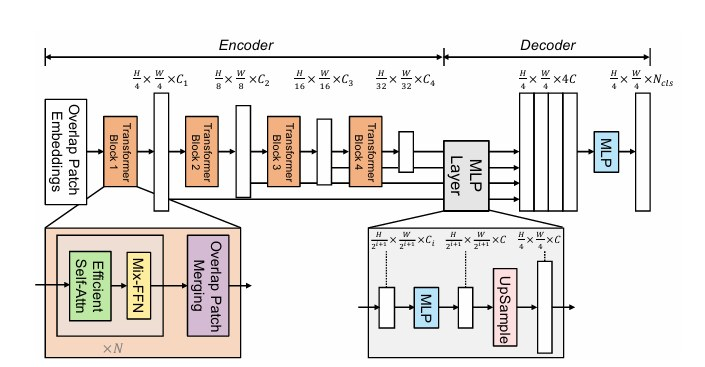
\includegraphics[width=\textwidth]{images/segformer_overview.jpg}
    \caption[ภาพรวมกระบวนการทำงานของ SegFormer]{ภาพรวมกระบวนการทำงานของ SegFormer (จาก \cite{xie2021segformersimpleefficientdesign})}
    \label{fig:proposed SegFormer}
\par\vspace{3pt}{\footnotesize\raggedright หมายเหตุ: SegFormer = Segmentation Transformer\par}
\end{figure}

\subsubsection{Hierarchical Transformer Encoder (ส่วนสกัดคุณลักษณะ)}
ตัวเข้ารหัสแปลงภาพเป็นคุณลักษณะ 4 ระดับความละเอียด
โดยใช้กลไกความสนใจตนเองแบบประหยัด (Efficient Self-Attention)
ซึ่งย่อความยาวลำดับของคีย์และค่าลงด้วยอัตราส่วน $R$
ทำให้ปริมาณการคำนวณลดจาก $\mathcal{O}(n^2)$ เหลือ $\mathcal{O}(n^2/R)$
ดังสมการที่~(\ref{eq:segformer_attn})
\begin{equation}
    \text{Attention}(Q, \hat{K}, V) = \text{Softmax}\!\left(\frac{Q\hat{K}^T}{\sqrt{d_\text{head}}}\right) V
    \label{eq:segformer_attn}
\end{equation}
\begin{vardef}
$Q$ & เมทริกซ์คิวรี (Query) คือคุณลักษณะของตำแหน่งที่กำลังพิจารณา \\
$\hat{K}$ & เมทริกซ์คีย์ (Key) ที่ถูกลดความยาวลำดับด้วยอัตราส่วน $R$ \\
$V$ & เมทริกซ์ค่า (Value) ที่ถูกดึงมารวมตามน้ำหนักความสนใจ \\
$d_\text{head}$ & มิติของหัวความสนใจ (Attention Head) ใช้ปรับสเกล \\
$n$ & จำนวนส่วนย่อยของภาพ เท่ากับ $HW/P^2$ เมื่อ $P$ คือขนาดของส่วนย่อย
\end{vardef}

\subsubsection{All-MLP Decoder (ส่วนทำนายผลลัพธ์)}
ตัวถอดรหัสรวมคุณลักษณะจากหลายความละเอียดผ่าน MLP เพื่อทำนายประเภทของทุกพิกเซล
จากนั้นสร้างหน้ากากแบบสองค่า (มีเฉพาะ 0 กับ 1) ของบริเวณที่สนใจ เช่น บริเวณผม
ตามสมการที่~(\ref{eq:segformer_binary})
\begin{equation}
    B(x, y) =
    \begin{cases}
        1 & \text{ถ้า } \arg\max_{c}\, M(x, y, c) = \text{``Hair''} \\
        0 & \text{ในกรณีอื่น}
    \end{cases}
    \label{eq:segformer_binary}
\end{equation}
\begin{vardef}
$B(x, y)$ & ค่าหน้ากากเส้นผม ณ พิกเซล $(x,y)$ (1 = เป็นผม) \\
$M(x, y, c)$ & คะแนนที่โมเดลทำนายว่าพิกเซล $(x,y)$ เป็นประเภท $c$ \\
$\arg\max_c$ & การเลือกประเภทที่มีคะแนนสูงสุด
\end{vardef}
ผู้พัฒนาฝึก SegFormer ด้วยค่าสูญเสียครอสเอนโทรปีรายพิกเซล ตามสมการที่~(\ref{eq:segformer_loss})
\begin{equation}
    \mathcal{L}_\text{seg} = -\sum_{x,y} \sum_{c=1}^{C} \mathbf{1}\!\left[y_{xy} = c\right] \log \hat{p}_{xy,c}
    \label{eq:segformer_loss}
\end{equation}
\begin{vardef}
$y_{xy}$ & ประเภทจริงของพิกเซล $(x,y)$ \\
$\hat{p}_{xy,c}$ & ความน่าจะเป็นที่โมเดลทำนายว่าพิกเซล $(x,y)$ เป็นประเภท $c$ \\
$C$ & จำนวนประเภททั้งหมด \\
$\mathbf{1}[\cdot]$ & ฟังก์ชันบ่งชี้ มีค่า 1 เมื่อเงื่อนไขเป็นจริง และ 0 ในกรณีอื่น
\end{vardef}
งานวิจัยนี้ใช้ SegFormer-B2 ที่ฝึกมาสำหรับแยกส่วนต่าง ๆ ของบุคคล
และรวมหน้ากากผมกับหน้ากากใบหน้าเป็นบริเวณที่อนุญาตให้ Diffusion แก้ไข
ตามสมการที่~(\ref{eq:m_edit}) ส่วนเสื้อผ้าและพื้นหลังจะไม่ถูกแก้ไข
\begin{equation}
    M_\text{edit}(x, y) = B_\text{hair}(x, y) \lor B_\text{face}(x, y)
    \label{eq:m_edit}
\end{equation}
\begin{vardef}
$M_\text{edit}$ & หน้ากากบริเวณที่อนุญาตให้แก้ไข \\
$B_\text{hair}, B_\text{face}$ & หน้ากากบริเวณผมและบริเวณใบหน้าจาก SegFormer \\
$\lor$ & การรวม (OR) คือเป็น 1 เมื่อพิกเซลอยู่ในบริเวณใดบริเวณหนึ่ง
\end{vardef}

% -----------------------------------------------------------
\subsection{การปรับปรุงคุณภาพภาพด้วย Stable Diffusion}
\label{sec:stablediffusion}
% -----------------------------------------------------------
Stable Diffusion~\cite{rombach2022highresolutionimagesynthesislatent} เป็นแบบจำลองดิฟฟิวชันในพื้นที่แฝง (Latent Diffusion Model: LDM)
ที่งานวิจัยนี้ใช้เป็นขั้นขัดเกลาภาพ (Post-processing) โดยรับภาพจาก HairFastGAN หรือ Barbershop
และหน้ากาก $M_\text{edit}$ แล้วเติมรายละเอียดของเส้นผมและผิวให้สมจริงขึ้น
ภาพที่~\ref{fig:stable_diffusion_arch} แสดงสถาปัตยกรรมของ Stable Diffusion ซึ่งแบ่งเป็น 3 ส่วน
ส่วนซ้าย (Pixel Space สีแดง) คือตัวเข้ารหัส $\mathcal{E}$ และตัวถอดรหัส $\mathcal{D}$ ที่แปลงภาพไปและกลับจากพื้นที่แฝง
ส่วนกลาง (Latent Space สีเขียว) คือกระบวนการดิฟฟิวชันที่ U-Net ลบสัญญาณรบกวนทีละขั้น
โดยมีบล็อก $Q$, $K$, $V$ เป็นจุดรับเงื่อนไข
และส่วนขวา (Conditioning สีเทา) คือแหล่งของเงื่อนไข เช่น ข้อความหรือแผนที่ความหมาย
ซึ่งถูกแปลงด้วยตัวเข้ารหัส $\tau_\theta$

\begin{figure}[H]
    \centering
    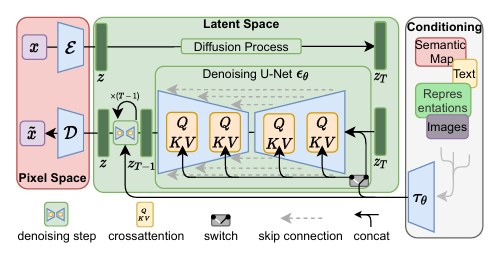
\includegraphics[width=0.8\textwidth]{images/sd_architecture.jpg}
    \caption[สถาปัตยกรรมและการทำงานภายในของ Stable Diffusion]{สถาปัตยกรรมและการทำงานของ Stable Diffusion ใน Latent Space (จาก \cite{rombach2022highresolutionimagesynthesislatent})}
    \label{fig:stable_diffusion_arch}
\end{figure}

\subsubsection{Perceptual Image Compression (การบีบอัดและคืนสภาพภาพ)}
ตัวเข้ารหัสอัตโนมัติแบบแปรผัน (Variational Autoencoder: VAE) บีบภาพให้เป็นข้อมูลแฝงที่เล็กลง 8 เท่าในแต่ละด้าน
และถอดรหัสกลับเป็นภาพ ตามสมการที่~(\ref{eq:sd_autoencoder})
การทำดิฟฟิวชันบนข้อมูลแฝงขนาดเล็กนี้แทนการทำบนพิกเซลโดยตรงช่วยลดการคำนวณลงมาก
\begin{equation}
    z = \mathcal{E}(x), \qquad \tilde{x} = \mathcal{D}(z)
    \label{eq:sd_autoencoder}
\end{equation}
\begin{vardef}
$x$ & ภาพนำเข้า \\
$\tilde{x}$ & ภาพที่สร้างคืนจากข้อมูลแฝง \\
$\mathcal{E}, \mathcal{D}$ & ตัวเข้ารหัส (Encoder) และตัวถอดรหัส (Decoder) \\
$z$ & ข้อมูลแฝงที่ถูกบีบอัดแล้ว (ภาพ $1024 \times 1024$ เหลือ $128 \times 128 \times 4$)
\end{vardef}
ภาพที่~\ref{fig:ldm_compression} อธิบายว่าทำไมจึงบีบอัดภาพได้
แกนนอนคืออัตราการเก็บข้อมูล (บิตต่อมิติ) และแกนตั้งคือความผิดเพี้ยนของภาพ
ช่วงซ้ายที่เส้นชันมาก (Semantic Compression) คือส่วนที่เก็บความหมายหลักของภาพ
ส่วนช่วงขวาที่เส้นเกือบแบน (Perceptual Compression) คือรายละเอียดที่ตาแทบมองไม่เห็นแต่ใช้ข้อมูลมาก
LDM จึงให้ Autoencoder ตัดส่วนหลังนี้ทิ้ง และให้ดิฟฟิวชันทำงานเฉพาะกับส่วนที่มีความหมาย

\begin{figure}[H]
    \centering
    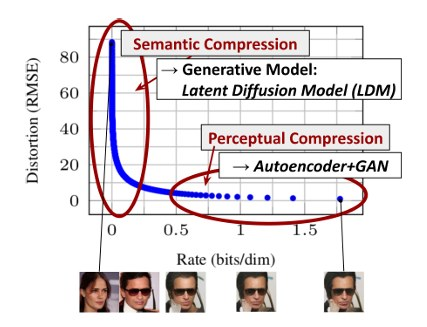
\includegraphics[width=0.5\textwidth]{images/ldm_compression.jpg}
    \caption[การบีบอัดเชิงการรับรู้และเชิงความหมายของ LDM]{การบีบอัดเชิงการรับรู้ (Perceptual Compression) และเชิงความหมาย (Semantic Compression) ของ Latent Diffusion Model (จาก \cite{rombach2022highresolutionimagesynthesislatent})}
    \label{fig:ldm_compression}
\par\vspace{3pt}{\footnotesize\raggedright หมายเหตุ: LDM = Latent Diffusion Model\par}
\end{figure}

\subsubsection{Denoising U-Net (กระบวนการลบสัญญาณรบกวน)}
แบบจำลองดิฟฟิวชัน~\cite{ho2020denoisingdiffusionprobabilisticmodels} เรียนรู้การลบสัญญาณรบกวนออกจากข้อมูลแฝงทีละขั้นเวลา
ระหว่างการฝึก ข้อมูลแฝง $z_0$ จะถูกผสมสัญญาณรบกวนตามสมการที่~(\ref{eq:forward_noise})
\begin{equation}
    z_t = \sqrt{\bar\alpha_t}\, z_0 + \sqrt{1 - \bar\alpha_t}\, \epsilon, \qquad \epsilon \sim \mathcal{N}(0, I)
    \label{eq:forward_noise}
\end{equation}
\begin{vardef}
$z_0$ & ข้อมูลแฝงของภาพที่ไม่มีสัญญาณรบกวน \\
$z_t$ & ข้อมูลแฝงที่ขั้นเวลา $t$ ซึ่งมีสัญญาณรบกวนปนอยู่ \\
$\bar\alpha_t$ & ตารางสัดส่วนของภาพเดิมที่เหลืออยู่ ลดจาก 1 ไปใกล้ 0 เมื่อ $t$ เพิ่มขึ้น \\
$\epsilon$ & สัญญาณรบกวนแบบเกาส์เซียน \\
$\mathcal{N}(0, I)$ & การแจกแจงปกติที่มีค่าเฉลี่ย 0 และความแปรปรวน 1
\end{vardef}
จากนั้นฝึก U-Net ให้ทายว่าสัญญาณรบกวนที่ใส่ลงไปมีค่าเท่าใด ด้วยสมการที่~(\ref{eq:sd_loss})
\begin{equation}
    \mathcal{L}_\text{LDM} = \mathbb{E}_{z,\;\epsilon,\;t}\Bigl[ \left\| \epsilon - \epsilon_\theta(z_t,\; t) \right\|^2_2 \Bigr]
    \label{eq:sd_loss}
\end{equation}
\begin{vardef}
$\mathcal{L}_\text{LDM}$ & ค่าความผิดพลาดกำลังสองเฉลี่ย (Mean Squared Error: MSE) ของการทายสัญญาณรบกวน \\
$\epsilon_\theta$ & เครือข่าย U-Net ที่มีพารามิเตอร์ $\theta$ ทำหน้าที่ทายสัญญาณรบกวน \\
$t$ & ขั้นเวลาที่สุ่มมาในการฝึก
\end{vardef}

\subsubsection{Cross-Attention Mechanism (การควบคุมด้วยข้อความ)}
กลไกความสนใจข้าม (Cross-Attention) เชื่อมข้อความสั่งงานเข้ากับการสร้างภาพ ตามสมการที่~(\ref{eq:sd_qkv})
และ~(\ref{eq:sd_crossattn}) เพื่อให้ U-Net สร้างรายละเอียดตามที่ข้อความกำหนด
\begin{equation}
    Q = W_Q \cdot \varphi(z_t), \quad K = W_K \cdot \tau_\theta(y), \quad V = W_V \cdot \tau_\theta(y)
    \label{eq:sd_qkv}
\end{equation}
\begin{equation}
    \text{CrossAttn}(Q, K, V) = \text{Softmax}\!\left(\frac{QK^T}{\sqrt{d}}\right) \cdot V
    \label{eq:sd_crossattn}
\end{equation}
\begin{vardef}
$\varphi(z_t)$ & คุณลักษณะของภาพภายใน U-Net ณ ขั้นเวลา $t$ \\
$y$ & ข้อความสั่งงาน (Prompt) \\
$\tau_\theta(y)$ & เวกเตอร์ของข้อความจากตัวเข้ารหัสข้อความ (CLIP Text Encoder) \\
$W_Q, W_K, W_V$ & เมทริกซ์น้ำหนักที่แปลงเป็นคิวรี คีย์ และค่า \\
$d$ & มิติของเวกเตอร์คีย์ ใช้ปรับสเกล
\end{vardef}
เมื่อรวมเงื่อนไขข้อความเข้ากับการลบสัญญาณรบกวน จะได้ฟังก์ชันสูญเสียตามสมการที่~(\ref{eq:sd_conditional_loss})
\begin{equation}
    \mathcal{L}_\text{LDM-Cond} = \mathbb{E}_{z,\;y,\;\epsilon,\;t}\Bigl[ \left\| \epsilon - \epsilon_\theta(z_t,\; t,\; \tau_\theta(y)) \right\|^2_2 \Bigr]
    \label{eq:sd_conditional_loss}
\end{equation}
\begin{vardef}
$\mathcal{L}_\text{LDM-Cond}$ & ค่าสูญเสียของ LDM แบบมีเงื่อนไข \\
$\epsilon_\theta(z_t, t, \tau_\theta(y))$ & สัญญาณรบกวนที่ U-Net ทายเมื่อได้รับเงื่อนไขข้อความ
\end{vardef}

\subsubsection{Inpainting, Strength, Classifier-Free Guidance และ Scheduler}
ในงานวิจัยนี้ Stable Diffusion ทำงานแบบเติมภาพเฉพาะบริเวณ (Inpainting)
ผ่าน \texttt{StableDiffusionInpaintPipeline} ของไลบรารี Diffusers ด้วยรุ่น Realistic Vision v5.1
ซึ่งเป็นรุ่นสร้างภาพทั่วไปที่ U-Net รับข้อมูลแฝงเพียง 4 ช่องสัญญาณ
ไม่ใช่รุ่นที่ฝึกมาเพื่องานเติมภาพโดยเฉพาะ ซึ่งรับ 9 ช่องสัญญาณ (เพิ่มข้อมูลแฝงของภาพเดิม 4 ช่อง และหน้ากาก 1 ช่อง)
เมื่อใช้รุ่น 4 ช่องสัญญาณ ไลบรารีจะควบคุมบริเวณที่แก้ไขด้วยการแทนค่าในทุกขั้นของการลบสัญญาณรบกวน
คือบริเวณนอกหน้ากาก $M_\text{edit}$ จะถูกแทนด้วยข้อมูลแฝงของภาพเดิมที่เติมสัญญาณรบกวนถึงระดับเดียวกัน
ส่วนบริเวณในหน้ากากใช้ค่าที่ U-Net เพิ่งลบสัญญาณรบกวน
ภาพจึงถูกวาดใหม่เฉพาะในหน้ากาก โดยยังใช้ส่วนที่เหลือของภาพเป็นบริบท
แต่ในตอนท้าย ตัวถอดรหัส $\mathcal{D}$ จะถอดรหัสทั้งภาพ บริเวณนอกหน้ากากจึงเปลี่ยนไปเล็กน้อยจากการบีบอัดแล้วคืนสภาพ
ภาพที่~\ref{fig:ldm_inpaint} แสดงตัวอย่างของ LDM ในงานวิจัยต้นฉบับ
คอลัมน์ซ้ายคือภาพนำเข้าที่มีกรอบสีแดงล้อมบริเวณที่จะแก้ไข
และคอลัมน์ขวาคือผลที่บริเวณนั้นถูกเติมใหม่ให้กลืนกับภาพเดิม ขณะที่ส่วนอื่นไม่เปลี่ยน

\begin{figure}[H]
    \centering
    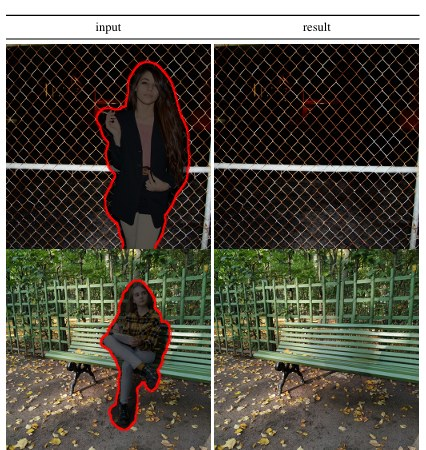
\includegraphics[width=0.45\textwidth]{images/ldm_inpaint_example.jpg}
    \caption[ตัวอย่างการ Inpainting ด้วย Latent Diffusion Model]{ตัวอย่างผลลัพธ์การ Inpainting ด้วย Latent Diffusion Model (จาก \cite{rombach2022highresolutionimagesynthesislatent})}
    \label{fig:ldm_inpaint}
\end{figure}

งานวิจัยนี้ใช้ดิฟฟิวชันแบบแรงต่ำ โดยกำหนดความแรง (Strength)
ซึ่งหมายถึงการเติมสัญญาณรบกวนให้ภาพเดิมตามสมการที่~(\ref{eq:forward_noise})
เพียงถึงขั้นเวลา $t = \text{strength} \times T$ แล้วจึงลบสัญญาณรบกวนออก
แทนที่จะเริ่มจากสัญญาณรบกวนล้วน เมื่อใช้ค่า 0.15 ภาพเดิมยังคงอยู่เกือบทั้งหมด
จึงเปลี่ยนเฉพาะพื้นผิวของเส้นผมและผิว นอกจากนี้ยังใช้การนำทางแบบไม่ใช้ตัวจำแนก
(Classifier-Free Guidance: CFG)~\cite{ho2022classifierfreediffusionguidance}
ซึ่งผสมผลทำนายเมื่อได้รับข้อความสั่งงาน กับผลทำนายเมื่อได้รับข้อความเชิงลบ (Negative Prompt)
ตามสมการที่~(\ref{eq:cfg}) เพื่อดันผลลัพธ์ให้ตรงกับข้อความสั่งงานและห่างจากสิ่งที่ไม่ต้องการ
\begin{equation}
    \hat\epsilon = \epsilon_\text{neg} + s \cdot \left(\epsilon_\text{prompt} - \epsilon_\text{neg}\right)
    \label{eq:cfg}
\end{equation}
\begin{vardef}
$\hat\epsilon$ & สัญญาณรบกวนที่ใช้จริงในการลบแต่ละขั้น \\
$\epsilon_\text{prompt}$ & สัญญาณรบกวนที่ U-Net ทายเมื่อได้รับข้อความสั่งงาน \\
$\epsilon_\text{neg}$ & สัญญาณรบกวนที่ U-Net ทายเมื่อได้รับข้อความเชิงลบ \\
$s$ & ค่านำทาง (Guidance Scale) งานวิจัยนี้ใช้ 2.5 ซึ่งเป็นค่าต่ำเพื่อไม่ให้ภาพเพี้ยน \\
$T$ & จำนวนขั้นเวลาทั้งหมดของกระบวนการดิฟฟิวชัน
\end{vardef}
สำหรับวิธีคำนวณแต่ละขั้นของการลบสัญญาณรบกวน (Scheduler) งานวิจัยนี้ใช้ Unified Predictor-Corrector (UniPC)~\cite{zhao2023unipcunifiedpredictorcorrectorframework}
ซึ่งใช้จำนวนขั้นน้อยแต่ยังได้ภาพคุณภาพดี เมื่อตั้งไว้ 30 ขั้นร่วมกับความแรง 0.15
จะลบสัญญาณรบกวนจริงประมาณ 4 ขั้น

% -----------------------------------------------------------
\subsection{การเรียนรู้แบบถ่ายโอนและการปรับจูนโมเดล}
\label{sec:finetune_theory}
% -----------------------------------------------------------
การปรับจูน (Fine-tuning) คือการนำโมเดลที่ผู้อื่นฝึกไว้แล้วมาฝึกต่ออีกเล็กน้อยด้วยข้อมูลของเราเอง
หรือที่เรียกว่าการเรียนรู้แบบถ่ายโอน (Transfer Learning)~\cite{yosinski2014transferablefeaturesdeepneural}
เปรียบเหมือนช่างตัดผมที่มีฝีมืออยู่แล้วมาเรียนเพิ่มเฉพาะเทคนิคใหม่ โดยไม่ต้องเริ่มเรียนตั้งแต่ศูนย์
โดยทั่วไปจะล็อกส่วนต้นของโมเดลไว้ และปรับเฉพาะบางส่วนด้วยอัตราการเรียนรู้ (Learning Rate: LR)
ซึ่งเป็นขนาดของการปรับน้ำหนักในแต่ละครั้ง โดยตั้งให้ต่ำมาก
เพื่อไม่ให้โมเดลลืมสิ่งที่เคยเรียนมา (Catastrophic Forgetting)
การฝึกหนึ่งรอบเริ่มจากคำนวณไปข้างหน้าจนได้ผลลัพธ์ แล้วคำนวณค่าสูญเสีย
หาอนุพันธ์ย้อนกลับ (Backpropagation) ด้วยกฎลูกโซ่
จากนั้นปรับน้ำหนักด้วยตัวปรับค่า Adaptive Moment Estimation (Adam)~\cite{kingma2017adammethodstochasticoptimization}
ซึ่งจำค่าเฉลี่ยเคลื่อนที่ของเกรเดียนต์และของเกรเดียนต์ยกกำลังสอง
เพื่อปรับขนาดก้าวให้เหมาะกับแต่ละพารามิเตอร์ ตามสมการที่~(\ref{eq:adam})
\begin{equation}
m_t = \beta_1 m_{t-1} + (1-\beta_1) g_t, \quad
v_t = \beta_2 v_{t-1} + (1-\beta_2) g_t^2, \quad
\theta_t = \theta_{t-1} - \eta \frac{\hat m_t}{\sqrt{\hat v_t} + \epsilon}
\label{eq:adam}
\end{equation}
\begin{vardef}
$\theta_t$ & ค่าพารามิเตอร์ (น้ำหนัก) ของโมเดลหลังการปรับรอบที่ $t$ \\
$g_t$ & เกรเดียนต์ของค่าสูญเสียเทียบกับพารามิเตอร์ในรอบที่ $t$ \\
$m_t, v_t$ & ค่าเฉลี่ยเคลื่อนที่ของเกรเดียนต์และของเกรเดียนต์ยกกำลังสอง \\
$\hat m_t, \hat v_t$ & ค่า $m_t$ และ $v_t$ ที่แก้ความเอนเอียงช่วงต้น (หารด้วย $1 - \beta^t$) \\
$\beta_1, \beta_2$ & ค่าคงที่ของค่าเฉลี่ยเคลื่อนที่ (0.9 และ 0.999) \\
$\eta$ & อัตราการเรียนรู้ \\
$\epsilon$ & ค่าคงที่ขนาดเล็กเพื่อกันการหารด้วยศูนย์
\end{vardef}

% -----------------------------------------------------------
\subsection{ตัวชี้วัดคุณภาพภาพ}
\label{sec:metrics_theory}
% -----------------------------------------------------------
งานวิจัยนี้ใช้ตัวชี้วัดหลายตัว เพื่อวัดแต่ละด้านแยกกัน
ด้านสีผมวัดในปริภูมิสี CIELAB (Lab) ซึ่งแยกความสว่าง ($L$ มีค่า 0--100)
ออกจากสี ($a$ คือแกนเขียวถึงแดง และ $b$ คือแกนน้ำเงินถึงเหลือง)
และออกแบบให้ระยะห่างของค่าสีใกล้เคียงกับความต่างที่ตามนุษย์รับรู้~\cite{doi:https://doi.org/10.1002/9781118653128.ch10}

ด้านทรงผมวัดด้วยค่าการทับซ้อนของบริเวณผมสองบริเวณ
ได้แก่ IoU และสัมประสิทธิ์ไดซ์ (Dice Coefficient)~\cite{milletari2016vnetfullyconvolutionalneural} ตามสมการที่~(\ref{eq:iou})
ทั้งสองค่ามีช่วง 0--1 โดย 1 หมายถึงทับกันพอดี
\begin{equation}
\mathrm{IoU} = \frac{\lvert A \cap B \rvert}{\lvert A \cup B \rvert}, \qquad
\mathrm{Dice} = \frac{2 \lvert A \cap B \rvert}{\lvert A \rvert + \lvert B \rvert}
\label{eq:iou}
\end{equation}
\begin{vardef}
$A$ & เซตของพิกเซลที่เป็นผมในภาพผลลัพธ์ \\
$B$ & เซตของพิกเซลที่เป็นผมในทรงเป้าหมาย \\
$\lvert \cdot \rvert$ & จำนวนพิกเซลในเซต \\
$\cap, \cup$ & ส่วนที่ทับกันและส่วนรวมของสองเซต
\end{vardef}

ด้านการคงส่วนที่ไม่ควรเปลี่ยน วัดด้วย SSIM~\cite{1284395} ตามสมการที่~(\ref{eq:ssim})
ซึ่งเทียบความสว่าง ความต่างของแสง และโครงสร้างในหน้าต่างย่อย ค่า 1.0 หมายถึงเหมือนกันทุกจุด
และวัดด้วยค่าความคลาดเคลื่อนสัมบูรณ์เฉลี่ย (Mean Absolute Error: MAE) ตามสมการที่~(\ref{eq:mae})
ซึ่งยิ่งต่ำยิ่งแปลว่าภาพเปลี่ยนน้อย
\begin{equation}
\mathrm{SSIM}(x,y) = \frac{(2\mu_x\mu_y + C_1)(2\sigma_{xy} + C_2)}{(\mu_x^2 + \mu_y^2 + C_1)(\sigma_x^2 + \sigma_y^2 + C_2)}
\label{eq:ssim}
\end{equation}
\begin{vardef}
$x, y$ & หน้าต่างย่อยของภาพสองภาพที่ตำแหน่งเดียวกัน \\
$\mu_x, \mu_y$ & ค่าเฉลี่ยความสว่างในหน้าต่าง \\
$\sigma_x^2, \sigma_y^2$ & ความแปรปรวน (ความต่างของแสง) ในหน้าต่าง \\
$\sigma_{xy}$ & ความแปรปรวนร่วม (ความคล้ายเชิงโครงสร้าง) \\
$C_1, C_2$ & ค่าคงที่ขนาดเล็กเพื่อกันการหารด้วยศูนย์
\end{vardef}
\begin{equation}
\mathrm{MAE} = \frac{1}{N} \sum_{p=1}^{N} \left\lvert x_p - y_p \right\rvert
\label{eq:mae}
\end{equation}
\begin{vardef}
$x_p, y_p$ & ค่าสีของพิกเซล $p$ ในภาพผลลัพธ์และภาพต้นฉบับ (ปรับเป็นช่วง 0--1) \\
$N$ & จำนวนพิกเซลในบริเวณที่วัด
\end{vardef}

ด้านคุณภาพภาพโดยรวม ใช้ Multi-scale Image Quality Transformer (MUSIQ)~\cite{ke2021musiqmultiscaleimagequality}
ซึ่งให้คะแนน 0--100 โดยไม่ต้องมีภาพอ้างอิง
ส่วนการบอกว่าผลต่างที่วัดได้เกิดขึ้นจริงหรือเกิดจากความบังเอิญ
งานวิจัยนี้ใช้ช่วงความเชื่อมั่น (Confidence Interval: CI) แบบบูตสแตรป (Bootstrap)~\cite{efron1994introduction}
คือสุ่มตัวอย่างจากข้อมูลเดิมแบบใส่คืนซ้ำหลายพันครั้ง คำนวณค่าเฉลี่ยทุกครั้ง
แล้วใช้เปอร์เซ็นไทล์ที่ 2.5 และ 97.5 ของค่าเฉลี่ยเหล่านั้นเป็นขอบของช่วงความเชื่อมั่น 95\%
ถ้าช่วงนี้ไม่ครอบคลุมเลข 0 แสดงว่าการเปลี่ยนแปลงนั้นไม่น่าเกิดจากความบังเอิญ
วิธีนี้ไม่ต้องสมมติรูปแบบการแจกแจงของข้อมูล แต่เมื่อข้อมูลมีน้อย ช่วงความเชื่อมั่นอาจยังไม่นิ่ง
จึงควรตีความเป็นผลเชิงสำรวจจากชุดตัวอย่างที่ศึกษาเท่านั้น
